\documentclass[cjk,slidestop,compress,mathserif,blue]{beamer}
%dvipdfm选项是关键,否则编译统统通不过
%beamer的颜色选项定义的是导航条和标题的颜色(即关键词structure的颜色)

%%%%%%%%%%%%%%%%仅限于XeTeX可使用的宏包%%%%%%%%%%%%%%%%%%%%%%%%%%%%
\usepackage{fontspec,xunicode,xltxtra,beamerthemesplit}
%\usepackage{beamerthemesplit}
\usepackage{handoutWithNotes}		%(讲义)在打印PPT的时候会留出给每一页做注释的部分
\usepackage{xeCJK}
\setCJKmainfont[BoldFont=黑体, ItalicFont=楷体, BoldItalicFont=仿宋]{黑体}
%\setsansfont[Mapping=tex-text]{Adobe 黑体 Std}
%如果装了Adobe Acrobat,可在font.conf中配置Adobe字体的路径以使用其中文字体
%也可直接使用系统中的中文字体如SimSun,SimHei,微软雅黑 等
%原来beamer用的字体是sans family;注意Mapping的大小写,不能写错

\usepackage{listings} 
\lstset{language=Matlab}%代码语言使用的是matlab 
\lstset{breaklines}%自动将长的代码行换行排版 
\lstset{extendedchars=false}%解决代码跨页时,章节标\dots

%%%%%%%%   确定标题和导航条结构的框架     %%%%%%%%%%%%
\usepackage{beamerthemeshadow}                       %
%\usepackage{beamerthemeclassic}%导航条色与背景色一致%
%%%%%%%%%%%%%%%%%%%%%%%%%%%%%%%%%%%%%%%%%%%%%%%%%%%%%%
\setbeamerfont{roman title}{size={}}
%\usepackage{CJK} % CJK 中文支持                                  %
\usepackage{amsmath,amsthm,amsfonts,amssymb,bm}
\usepackage{bbding}
\usepackage{mathrsfs}
\usepackage{xcolor}                                        %使用默认允许使用颜色
\usepackage{hyperref} 
\usepackage{graphicx}
\usepackage{subfigure}           %图片跨页
\usepackage{animate}		 %插入动画
\usepackage{tikz}		 %绘图工具
\usepackage{caption}
\captionsetup{font=footnotesize}

%\usepackage[version=3]{mhchem}		%化学公式
\usepackage{chemformula}
\usepackage{chemfig}		%化学公式

\usepackage{multirow}
\usepackage{makecell}		%允许单元格内换行

\usepackage[dvipdfmx]{movie15_dvipdfmx} %插入视频
%\usepackage{handoutWithNotes}		%(讲义)在打印PPT的时候会留出给每一页做注释的部分
%\pgfpagesuselayout{1 on 1 with notes landscape}[a4paper,border shrink=5mm]

%%%%%%%%%%%%%%%%%%%%%%BIBTEX 引用参考文献%%%%%%%%%%%%%%%%%%%%%%%%%%%%%%%%%%%%%%%%%%%%%%%%
%\usepackage{filecontents}
%\begin{filecontents*}{main.bib}
%@techreport{2012FracfocusChemical,
%  author = {FracFocus,},
%  howpublished = {\url{http://fracfocus.org/water-protection/drilling-usage}},
%  institution = {The Ground Water Protection Council and Interstate Oil and Gas
%  Compact Commission},
%  month = {feb},
%  title = {{Chemical Use In Hydraulic Fracturing}},
%  year = {2012}
%}
%\end{filecontents*}
%\usepackage[backend=bibtex,sorting=none]{biblatex}
%%\usepackage[backend=biber,style=authoryear]{biblatex}
%\addbibresource{main.bib} %BibTeX数据文件及位置

%\usepackage[numbers,sort&compress]{natbib} %紧密排列             %
\usepackage[sectionbib]{chapterbib}        %每章节单独参考文献   %
\usepackage{hypernat}                                                                         %
\setbeamertemplate{bibliography item}[text] %参考文献前标注[]
%\usepackage[dvipdfm,bookmarksopen=true,pdfstartview=FitH,CJKbookmarks]{hyperref}		%
\hypersetup{bookmarksnumbered,colorlinks,linkcolor=brown,citecolor=blue,urlcolor=red}         %
%参考文献含有超链接引用时需要下列宏包,注意与natbib有冲突        %
%\usepackage[dvipdfm]{hyperref}                                  %
%\usepackage{hypernat}                                           %
\newcommand{\upcite}[1]{\hspace{0ex}\textsuperscript{\cite{#1}}} %

%\usepackage{marvosym} %插入各种符号

%\useoutertheme{smoothbars}
\useinnertheme[shadow=true]{rounded}
\usetheme{Berkeley}                                          %主题式样
%\usetheme{Luebeck}

\usecolortheme{lily}                                        %颜色主题式样

\usefonttheme{professionalfonts}                           %字体主题样式宏包

%\beamertemplatetransparentcoveredhigh                      %使所有被隐藏的文本高度透明
\beamertemplatetransparentcovereddynamicmedium             %使所有被隐藏的文本完全透明,动态,动态的范围很小
\mode<presentation>
%\beamersetaveragebackground{gray}                          %设置背景颜色(单一色) 
\beamertemplateshadingbackground{green!10}{red!5}         %设置背景颜色(渐变色)

%i放置单位logo
%\logo{
\includegraphics[width=1.6cm,height=0.35cm]{Figures/BCC_logo-1.png}}	%简单设置logo

%\pgfdeclareimage[width=3.5cm]{logoname}{Figures/BCC_logo-1.png}		%logo置于左侧微调
%\logo{\pgfuseimage{logoname}{\vspace{0.2cm}\hspace*{-2.0cm}}}

%在指定位置精确放置logo
\usepackage{tikz}
\usepackage{beamerfoils}
\usepackage{pgf}
%\logo{\pgfputat{\pgfxy(9.99,0.00)}{
\includegraphics[height=0.75cm,viewport=5 2 520 120,clip]{Figures/BCC_logo-1.png}}}
%\logo{\pgfputat{\pgfxy(10.45,0.00)}{
\includegraphics[height=0.65cm,viewport=6.5 39 264 102,clip]{Figures/BCC_logo-2.jpg}}}
\logo{\pgfputat{\pgfxy(11.68,0.15)}{
\includegraphics[height=1.01cm,viewport=0 0 140 120,clip]{Figures/BCC_logo-1.png}}\pgfputat{\pgfxy(10.502,-0.218)}{
\includegraphics[height=0.369cm,viewport=140 0 540 120,clip]{Figures/BCC_logo-1.png}}}
%\logo{\pgfputat{\pgfxy(11.68,0.15)}{
\includegraphics[height=0.95cm,viewport=0 0 510 360,clip]{Figures/Logo_Gainstrong.png}}\pgfputat{\pgfxy(10.333,-0.195)}{
\includegraphics[height=0.35cm,viewport=530 70 1100 218,clip]{Figures/Logo_Gainstrong.png}}}
%\logo{\pgfputat{\pgfxy(10.28,0.00)}{
\includegraphics[height=0.95cm,viewport=0 0 1100 360,clip]{Figures/Logo_Gainstrong.png}}}
%\logo{\pgfputat{\pgfxy(11.68,0.15)}{
\includegraphics[height=0.95cm,viewport=0 0 510 360,clip]{Figures/Logo_Gainstrong.png}}\pgfputat{\pgfxy(10.333,-0.195)}{
\includegraphics[height=0.35cm,viewport=530 70 1100 218,clip]{Figures/Logo_Gainstrong.png}}}
%\MyLogo{
%	\pgfputat{\pgfxy(-50,-50)}{\pgfbox[right,base]{
\includegraphics[height=1cm]{Figures/BCC_logo-1.png}}}

%logo作为背景放置
%\setbeamertemplate{background}{
%	\pgfputat{\pgfxy(6.5,-0.5)}{\pgfbox[left,top]{\pgfimage[height=1.1cm]{Figures/BCC_logo-1.png}}}}

%\logo{}									%不显示logo

\begin{document}
%\begin{CJK*}{GBK}{song}
%\begin{CJK*}{GBK}{kai}
%beamer下不能用\songyi、\zihao等命令!
%\graphicspath{Figures/}

%\renewcommand{\figurename}{\tiny\CJKfamily{hei} 图.}
\renewcommand{\figurename}{\tiny{\bf Fig}.}
%\renewcommand{\tablename}{\tiny\CJKfamily{hei} 表.}
\renewcommand{\tablename}{\tiny{\bf Tab}.}
%\renewcommand{\tablename}{\tiny\CJKfamily{hei} 表.}
%\renewcommand{\thesubfigure}{\roman{subfigure}}  %\makeatletter 子图标记罗马字母
\renewcommand{\thesubfigure}{\tiny(\alph{subfigure})}  %\makeatletter 子图标记英文字母
%\renewcommand{\thesubfigure}{}  \makeatletter %子图无标记

%%%%%%%%%%%%%%%%%%%%%%%%%%%%%%% Latex 的 tikz 绘图 %%%%%%%%%%%%%%%%%%%%%%%%%%%%%%%%%%%%%%%%%%%
%\begin{tikzpicture}
%    % 引入图片
%    \node[anchor=south west,inner sep=0] (image) at (0,0) {\includegraphics[width=0.9\textwidth]{Mycena_interrupta.jpg}};
%
%    \begin{scope}[x={(image.south east)},y={(image.north west)}]
%        % 建立相对坐标系
%        \draw[help lines,xstep=.1,ystep=.1] (0,0) grid (1,1);
%        \foreach \x in {0,1,...,9} { \node [anchor=north] at (\x/10,0) {0.\x}; }
%        \foreach \y in {0,1,...,9} { \node [anchor=east] at (0,\y/10) {0.\y}; }
%        % 作图命令
%        \draw[red, ultra thick, rounded corners] (0.62,0.65) rectangle (0.78,0.75);
%    \end{scope}
%\end{tikzpicture}
%%%%%%%%%%%%%%%%%%%%%%%%%%%%%%%%%%%%%%%%%%%%%%%%%%%%%%%%%%%%%%%%%%%%%%%%%%%%%%%%%%%%%%%%%%%%%%

%-------------------------------PPT Title-------------------------------------
\title{材料自动计算流程与面向催化材料的平台设计}
%-----------------------------------------------------------------------------

%----------------------------Author & Date------------------------------------
%\author[\textrm{Jun\_Jiang}]{姜\;\;骏\inst{}} %[]{} (optional, use only with lots of authors)
\author[]{北京市计算中心\;云平台\:姜骏}
% - Give the names in the same order as the appear in the paper.
% - Use the \inst{?} command only if the authors have different
%   affiliation.
\institute[BCC]{\inst{}%
% \vskip -20pt 北京市计算中心
}
\date[\today] % (optional, should be abbreviation of conference name)
{	%{\fontsize{6.2pt}{4.2pt}\selectfont{\textcolor{blue}{E-mail:~}\url{jiangjun@bcc.ac.cn}}}
\vskip 1 pt {\fontsize{8.2pt}{6.2pt}\selectfont{%北京理工大学%报告地点
	\vskip 2 pt \textrm{2021-05-24}}}
}

% - Either use conference name or its abbreviation
% - Not really information to the audience, more for people (including
%   yourself) who are reading the slides online

\subject{}
% This is only inserted into the PDF information catalog. Can be left
% out.
\frame
{
%	\frametitle{\fontsize{9.5pt}{5.2pt}\selectfont{\textcolor{orange}{“第一届材料\&科学青年峰会会议”}}}
\titlepage
}
%-----------------------------------------------------------------------------

%------------------------------------------------------------------------------列出全文 outline ---------------------------------------------------------------------------------
\section*{}
\frame[allowframebreaks]
{
  \frametitle{Outline}
%  \frametitle{\textcolor{mycolor}{\secname}}
  \tableofcontents%[current,currentsection,currentsubsection]
}
%在每个section之前列出全部Outline
%类似的在每个subsection之前列出全部Outline是\AtBeginSubsection[]
%\AtBeginSection[]
%{
%  \frame<handout:0>%[allowframebreaks]
%  {
%    \frametitle{Outline}
%%全部Outline中,本部分加亮
%    \tableofcontents[current,currentsection]
%  }
%}

%------------------------------------------------------------------------------PPT main Body------------------------------------------------------------------------------------
\small
%\section{引言}
\frame
{
	\frametitle{科学研究的范式变更}
\begin{figure}[h!]
\vspace*{-0.18in}
\centering
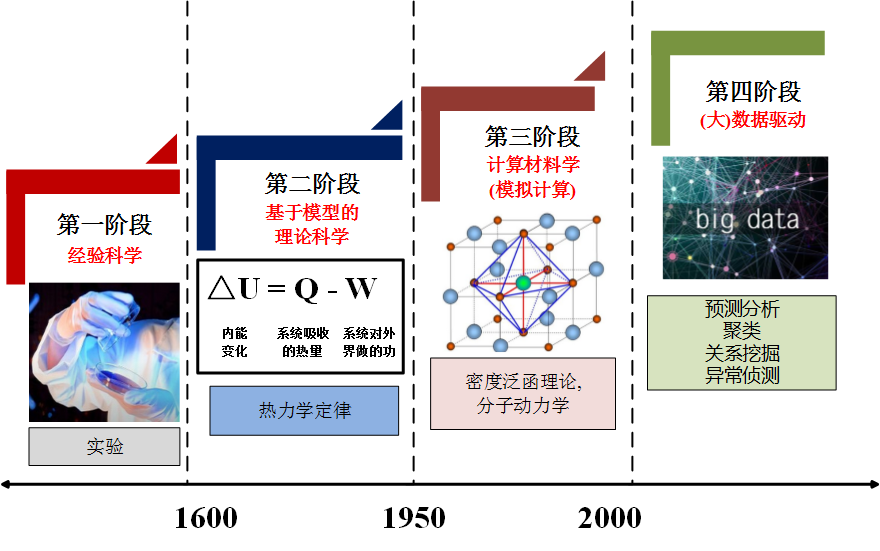
\includegraphics[width=4.05in]{Figures/Four_Model.png}
%\caption{\tiny \textrm{Pseudopotential for metallic sodium, based on the empty core model and screened by the Thomas-Fermi dielectric function.}}%(与文献\cite{EPJB33-47_2003}图1对比)
\label{Four_Model}
\end{figure}
}

\frame
{
	\frametitle{材料模拟的基本思想和方法}
\begin{figure}[h!]
\vspace*{-0.20in}
\centering
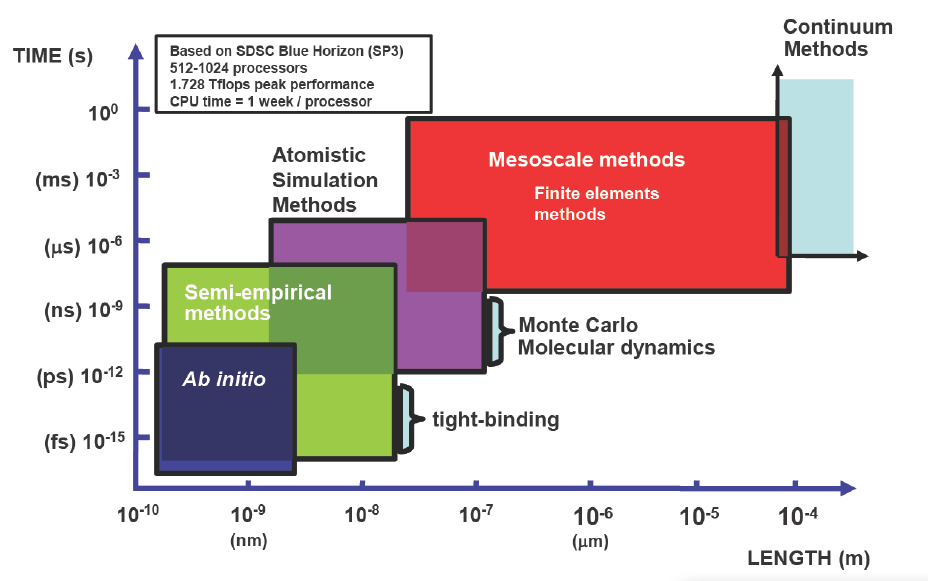
\includegraphics[height=2.20in,width=3.45in]{Figures/Multi-Scale-6.png}
\vskip 0.05pt
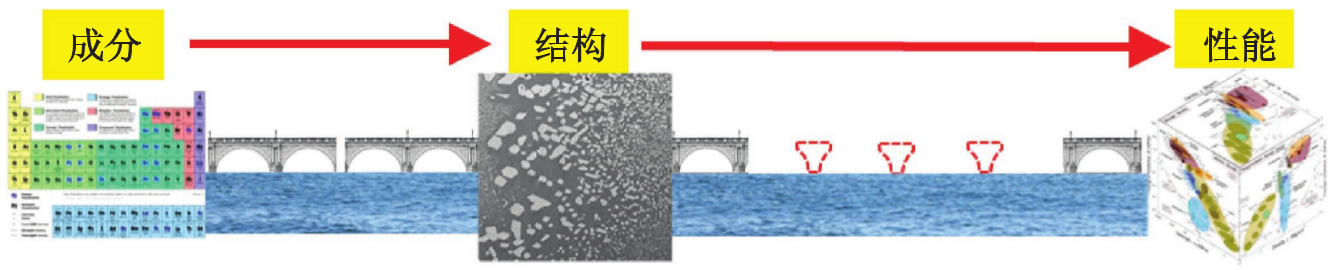
\includegraphics[height=0.80in,width=4.05in]{Figures/MGE-2.png}
%\caption{\tiny \textrm{Pseudopotential for metallic sodium, based on the empty core model and screened by the Thomas-Fermi dielectric function.}}%(与文献\cite{EPJB33-47_2003}图1对比)
\label{Multi-Scale}
\end{figure}
}

%\frame
%{
%	\frametitle{材料基因工程}
%\begin{figure}[h!]
%\vspace*{-0.18in}
%\centering
%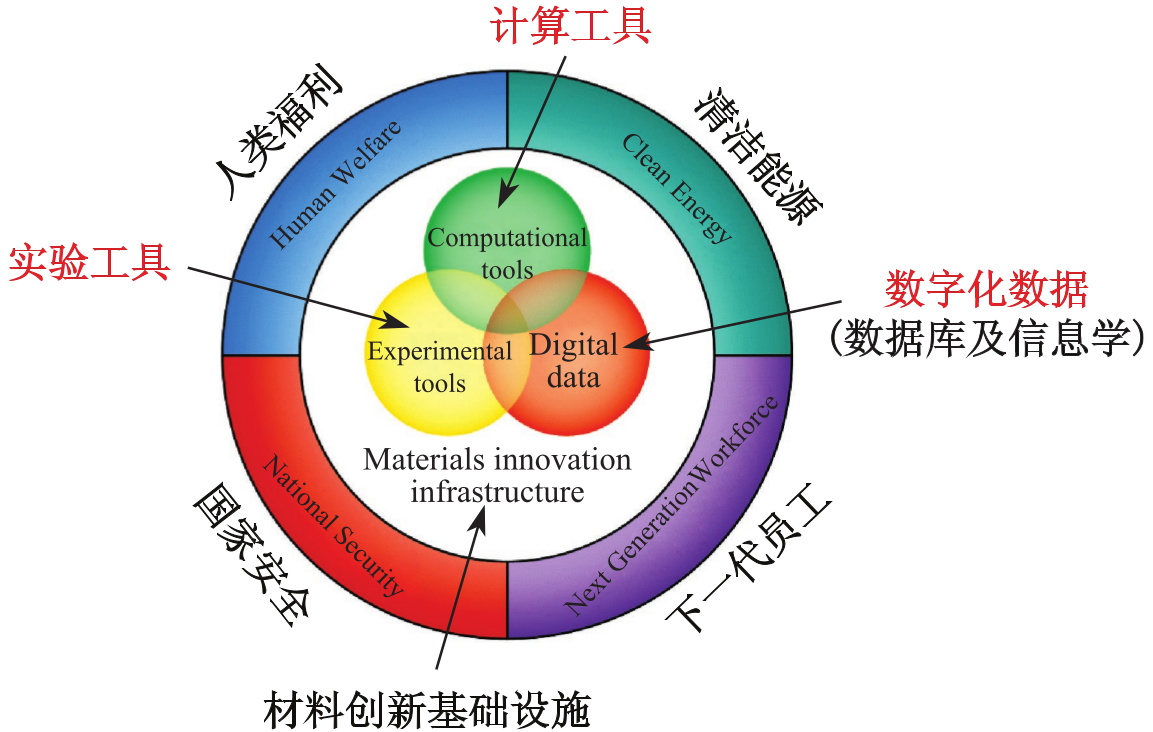
\includegraphics[height=2.55in,width=4.05in]{Figures/MGE.png}
%%\caption{\tiny \textrm{Pseudopotential for metallic sodium, based on the empty core model and screened by the Thomas-Fermi dielectric function.}}%(与文献\cite{EPJB33-47_2003}图1对比)
%\label{MGE}
%\end{figure}
%}
\section{密度泛函理论}
%\subsection{密度泛函理论}       %Bookmark
\frame                               %
{
\frametitle{密度泛函理论(\textrm{DFT})} %Slide Page Title
%   \secname
与传统的量子力学方法不同,密度泛函理论的基本变量是体系的基态电子密度。%通过体系的电子密度而非波函数确定体系的基态能量。
\begin{itemize}%[+-| alert@+>]
	\item 密度泛函理论的基石:\textrm{Hohenberg-Kohn}定理\upcite{PR136-B864_1964}
\vskip 5pt
\begin{itemize}%[+-| alert@+>]
   \setlength{\itemsep}{8pt}
 \item $E[\rho]=F_{\mathrm{HK}}[\rho]+\displaystyle\int\rho(\vec{r})v(\vec{r})\textrm{d}\vec{r}$ \\
\vskip 5pt 其中$F_{\mathrm{HK}}[\rho]=\underset{\Psi\to\rho}{\mathrm{Min}}\langle\Psi[\rho]|\hat{T}+\hat{W}|\Psi[\rho]\rangle$
是普适的泛函表达式。%,指明多电子体系的基态性质与基态密度间存在一一对应关系
     \textrm{\small{第一定理表明多电子体系的性质完全由体系的基态密度决定}}
   \item 如果$\tilde\Psi\neq\Psi$,
     $E[\tilde\rho]\geqslant E[\rho_0]$\\
     \textrm{\small{第二定理指出基态总能量泛函在体系基态电子密度处取极小值}}
   \end{itemize}
%\textrm{\small{第二定理指出基态总能量泛函在体系基态电子密度处取极小值}}
\vskip 8pt
 \item 密度泛函理论的优越性:用密度($\rho$)代替波函数($\Psi$)描述体系
\vskip 5pt
 \item 密度泛函理论的困难:能量密度泛函的精确形式未知
   \end{itemize}
}

\frame                               %
{
\frametitle{密度泛函理论(\textrm{DFT})}
\textrm{Kohn-Sham}方程\upcite{PR140-A1133_1965}:无相互作用体系+交换-相关能的贡献
$$(T_S+V_{e\!f\!f})|\varphi_i\rangle=\varepsilon_i|\varphi_i\rangle,\quad i=1,\cdots,N,\cdots$$
其中$T_S=-\dfrac12\nabla^2$~~是无相互作用体系的动能
\begin{displaymath}
	\begin{aligned}
		V_{e\!f\!f}(\vec r)=&V_{ext}(\vec r)+\displaystyle\int w(\vec r,\vec r\,')\rho(\vec r\,')\mathrm{d}\vec r\,'+V_{\mathrm{XC}}[\rho]\\
=&\displaystyle\int\dfrac{\rho(\vec r\,')}{|\vec r-\vec r^{\prime}|}\mathrm{d}\vec r\,'+V_{ext}(\vec r)+V_{\mathrm{XC}}[\rho]
	\end{aligned}
\end{displaymath}
$V_{ext}(\vec r)$是电子体系与外部的电荷或磁场相互作用\\
$V_{\mathrm{XC}}[\rho]=\dfrac{\delta E_{\mathrm{XC}}}{\delta\rho(\vec r)}$称为交换-相关势
\vskip 10pt
\textrm{Kohn-Sham}方程是形式上的单粒子方程
\vskip 6pt
\textrm{Kohn-Sham}方程的实质:\\\textcolor{red}{将动能泛函的主要部分分离出来,剩余部分放在交换-相关能中}
}

\frame
{
	\frametitle{\textrm{DFT-SCF}}
\begin{figure}[h!]
\centering
\vspace*{-0.25in}
\hspace*{-0.80in}
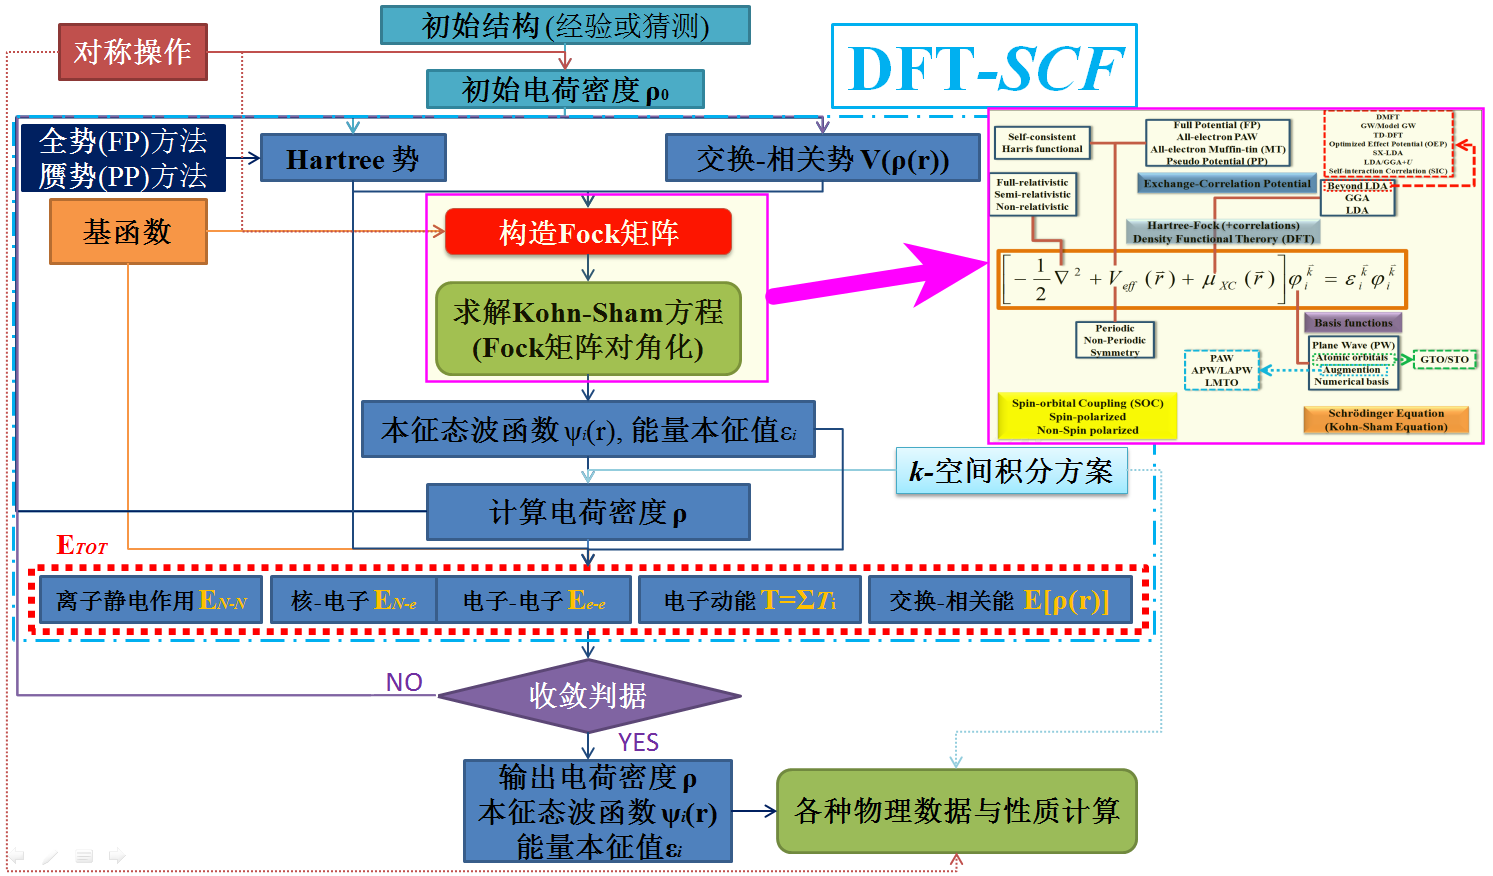
\includegraphics[height=2.80in,width=4.95in,viewport=5 3 1490 870,clip]{Figures/DFT-SCF_2.png}
%\caption{\tiny \textrm{Pseudopotential for metallic sodium, based on the empty core model and screened by the Thomas-Fermi dielectric function.}}%(与文献\cite{EPJB33-47_2003}图1对比)
\label{DFT-SCF-2}
\end{figure}
}

\section{自动流程框架与甲烷催化研究}
\frame
{
	\frametitle{计算主体框架的基本构想}
	\begin{itemize}
		\item 统一的高通量自动流程的数据格式
		\item 自动执行的多尺度、高通量计算流程,实现多组元材料体系从微观到宏观的结构、物性和服役行为的全链条多尺度集成计算
		\item 多尺度、高通量、高并发计算过程中不同计算任务间的高效信息传递、储存
		\item 规范定义不同模块间的I/O接口,搭建集成计算环境框架
	\end{itemize}
\begin{figure}[h!]
\centering
\vspace*{-0.2in}
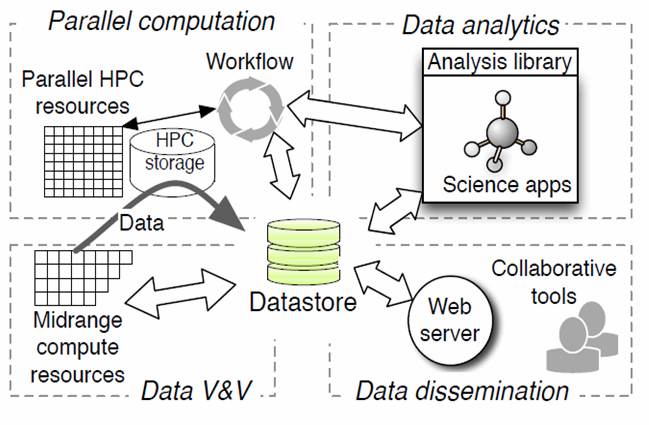
\includegraphics[height=1.3in,width=2.0in,viewport=0 0 680 460,clip]{Figures/Parallel_computation.png}
\caption{\fontsize{5.2pt}{2.5pt}\selectfont{\textrm{High throughput architecture. The datastore serves all four functions, clockwise from upper-left:~Parallel computation, Data analytics, Data dissemination, and Data validation and verification. Ref\cite{unpublished}}}}%
\label{parallel_computation}
\end{figure} 
}

\frame
{
	\frametitle{国外已有的计算平台}
\begin{figure}[h!]
\centering
\vspace{-15.5pt}
\subfigure[\fontsize{7.5pt}{6.2pt}\selectfont{\textrm{Auto-FLOW (AFLOW)}\upcite{CMS58-227_2012}}]{
\label{AFLOW_data_flow}
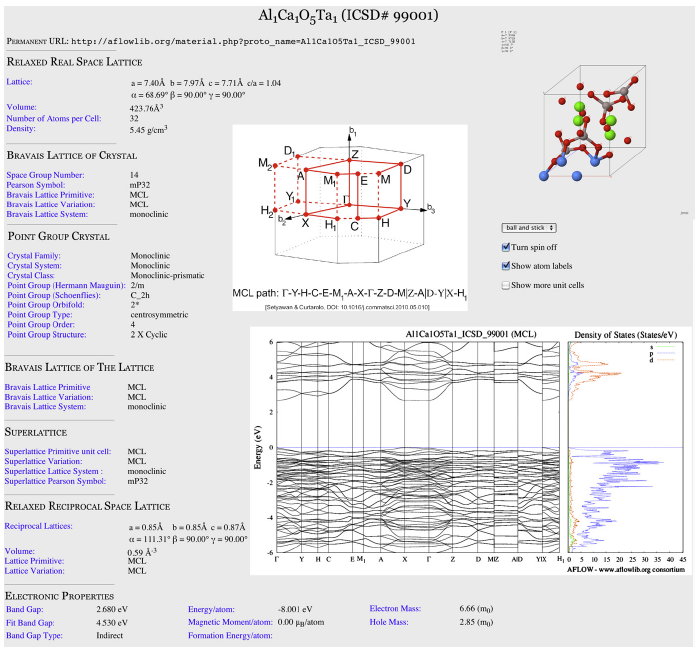
\includegraphics[height=1.2in,width=1.6in,viewport=0 0 720 660,clip]{Figures/AFLOW_database.png}}
\subfigure[\fontsize{7.5pt}{6.2pt}\selectfont{\textrm{Material Project (MP)}\upcite{CMS97-209_2015}}]{
\label{MP_commp_infrastructure}
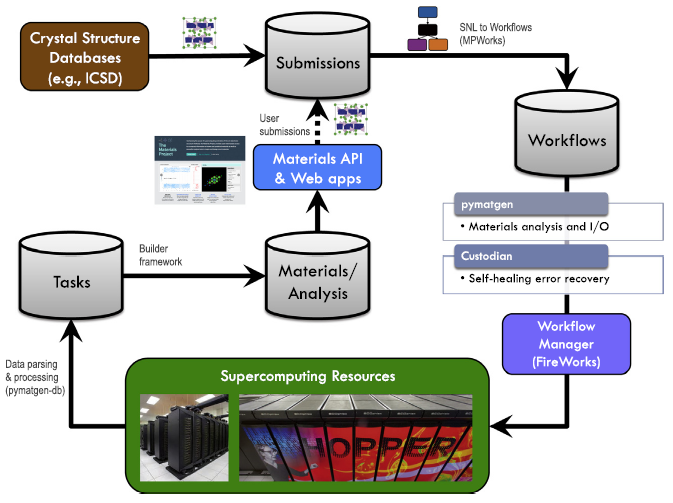
\includegraphics[height=1.2in,width=1.7in,viewport=0 0 670 530,clip]{Figures/MP_comp_infrastructure.png}}
\subfigure[\fontsize{3.5pt}{3.2pt}\selectfont{\textrm{Quantum Materials Informatics Project (QMIP)}\upcite{url_QMIP}}]{
\label{QMIP_Shame}
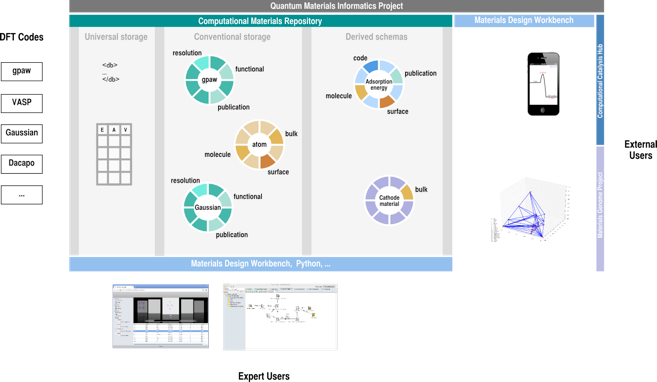
\includegraphics[height=1.2in,width=1.7in,viewport=0 0 670 420,clip]{Figures/QMIP_shame.png}}
\subfigure[\fontsize{6.5pt}{5.2pt}\selectfont{\textrm{Clean Energy Project (CEP)}\upcite{JPCL2-2241_2011}}]{
\label{CEP_structure_flow}
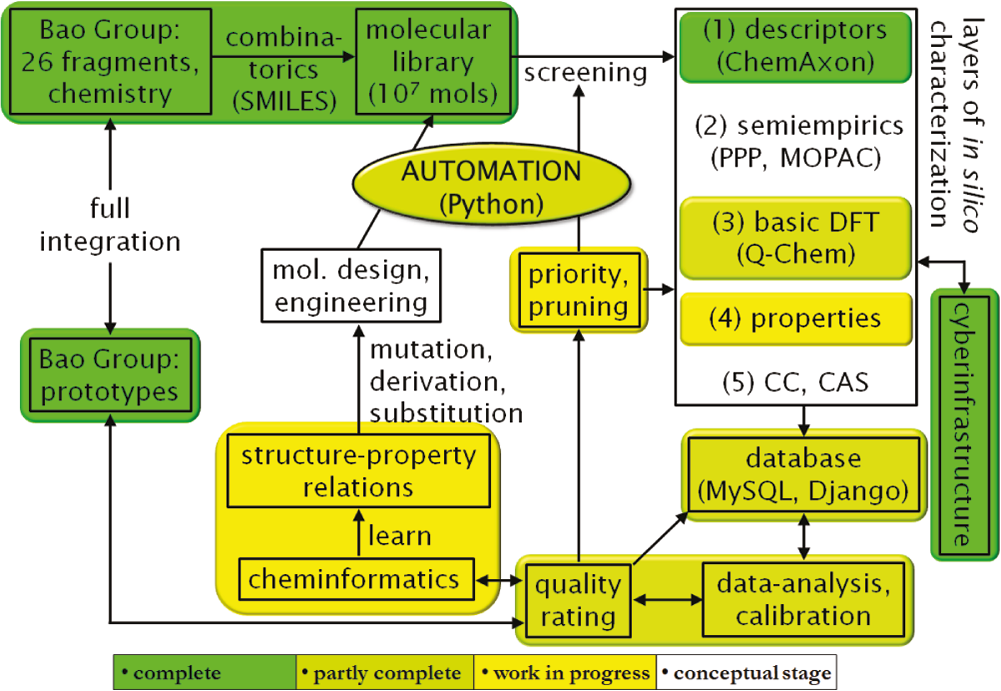
\includegraphics[height=1.2in,width=1.6in,viewport=0 0 1020 730,clip]{Figures/CEP_structure_flow.png}}
%\caption{}%
\label{Auto_Flow_Platform}
\end{figure}
}

%\frame
%{
%	\frametitle{\textrm{计算平台}}
%\begin{figure}[h!]
%\centering
%\vspace*{-0.2in}
%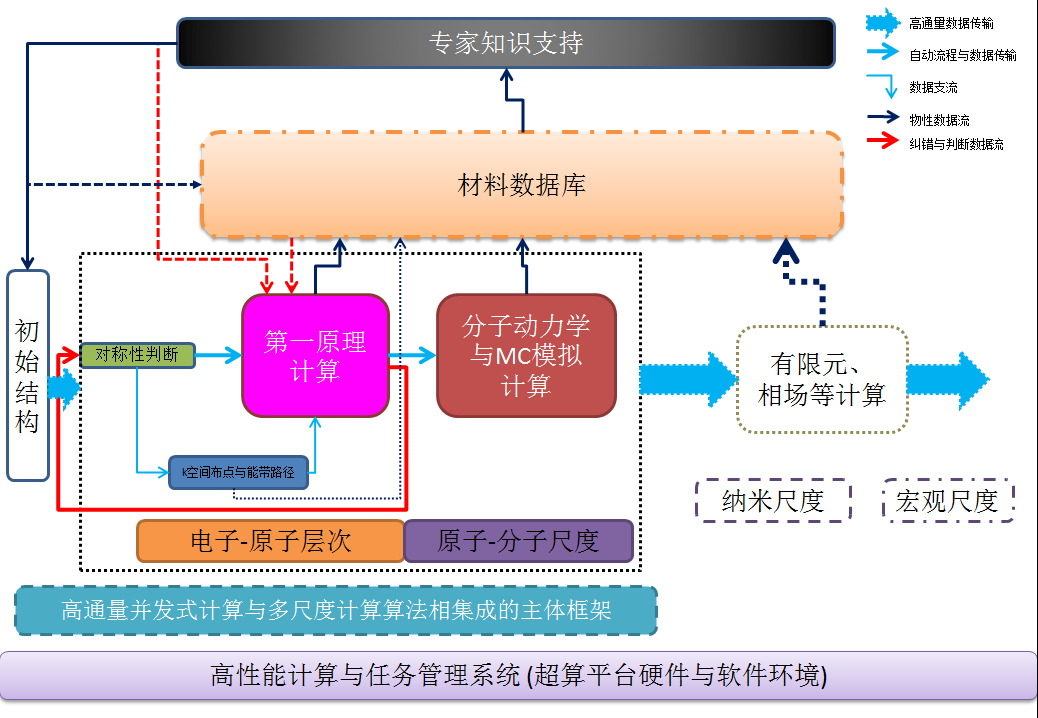
\includegraphics[height=2.6in,width=3.6in,viewport=0 0 1038 730,clip]{Figures/Auto_Flow.png}
%\caption{\fontsize{7.2pt}{4.2pt}\selectfont{\textrm{The schematic framework and platform of our project.}}}%
%\label{Auto_Flow}
%\end{figure} 
%}
%
\frame
{
	\frametitle{\textrm{基于ASE设计的多尺度计算}}
\begin{figure}[h!]
\centering
\vspace*{-0.2in}
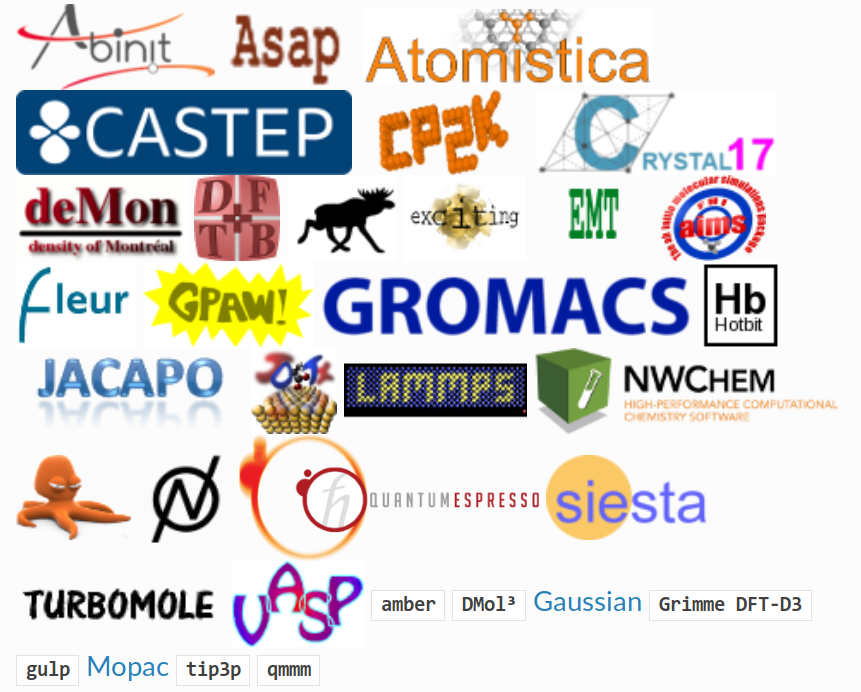
\includegraphics[height=2.1in,width=2.5in,viewport=0 0 638 530,clip]{Figures/ASE_calculator.png}
\caption{\fontsize{7.2pt}{4.2pt}\selectfont{\textrm{The integrated calculator in ASE (Atomic Simulation Environment).}}}%
\label{Logo_QM-MM}
\end{figure} 
}

\frame
{
	\frametitle{\textrm{计算平台的作业自动提交:~基于\textrm{ASE}}}
\begin{figure}[h!]
\centering
\vspace*{-0.2in}
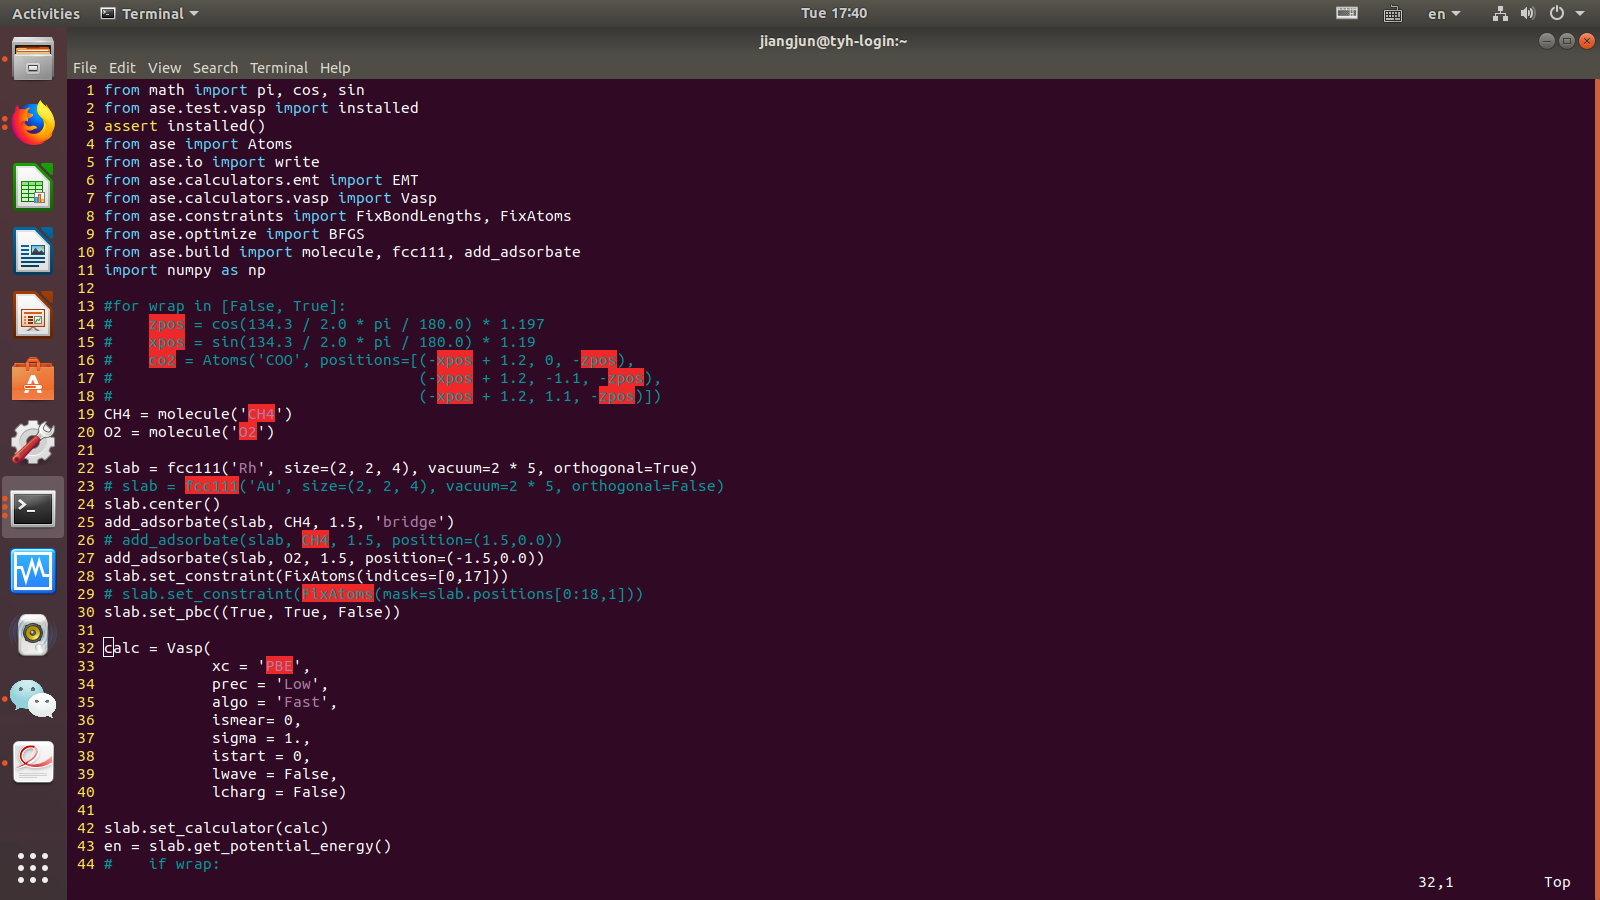
\includegraphics[height=3.1in,width=2.5in,viewport=75 0 725 820,clip]{Figures/ASE_app.png}
%\caption{\fontsize{7.2pt}{4.2pt}\selectfont{\textrm{The integrated calculator in ASE (Atomic Simulation Environment).}}}%
\label{ASE_app}
\end{figure} 
}

\frame
{
	\frametitle{\textrm{计算平台的结果展示:~基于\textrm{Pymatgen}}}
\begin{figure}[h!]
\centering
\vspace*{-0.2in}
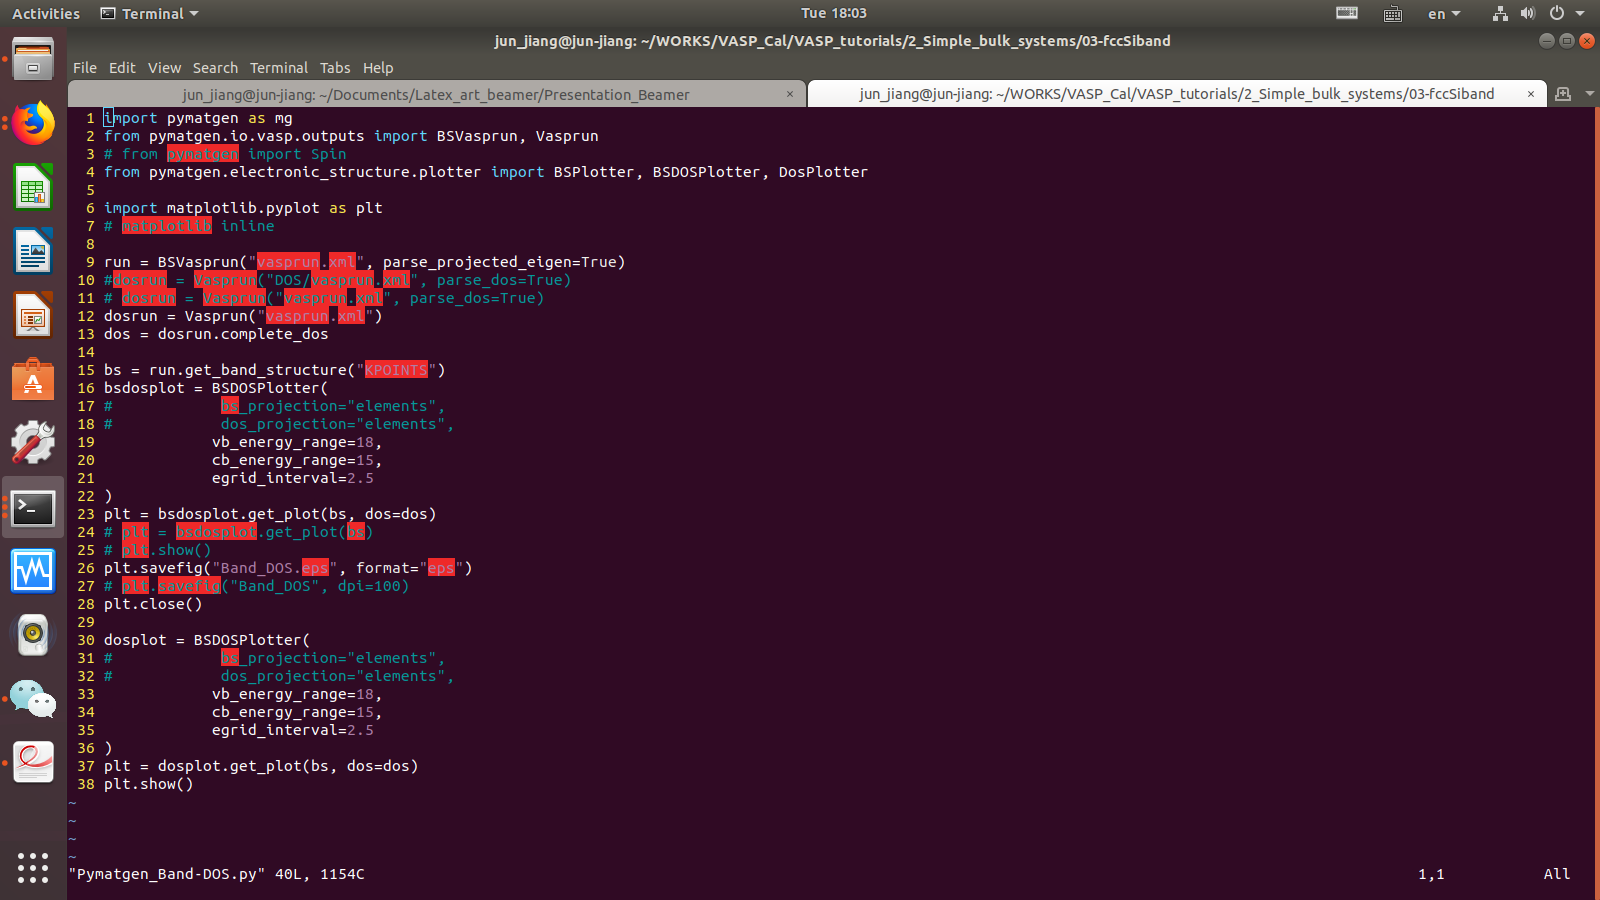
\includegraphics[height=3.1in,width=3.6in,viewport=73 80 880 790,clip]{Figures/Pymatgen_app.png}
%\caption{\fontsize{7.2pt}{4.2pt}\selectfont{\textrm{The integrated calculator in ASE (Atomic Simulation Environment).}}}%
\label{Pymatgen_app}
\end{figure} 
}

\frame
{
	\frametitle{\textrm{结果示例:~\textrm{FCC-Si}}}
	算例来源:\\\fontsize{7.5pt}{6.2pt}\selectfont{\url{http://cms.mpi.univie.ac.at/wiki/index.php/Fcc_Si_bandstructure}}
\begin{figure}[h!]
\centering
\vspace*{-0.1in}
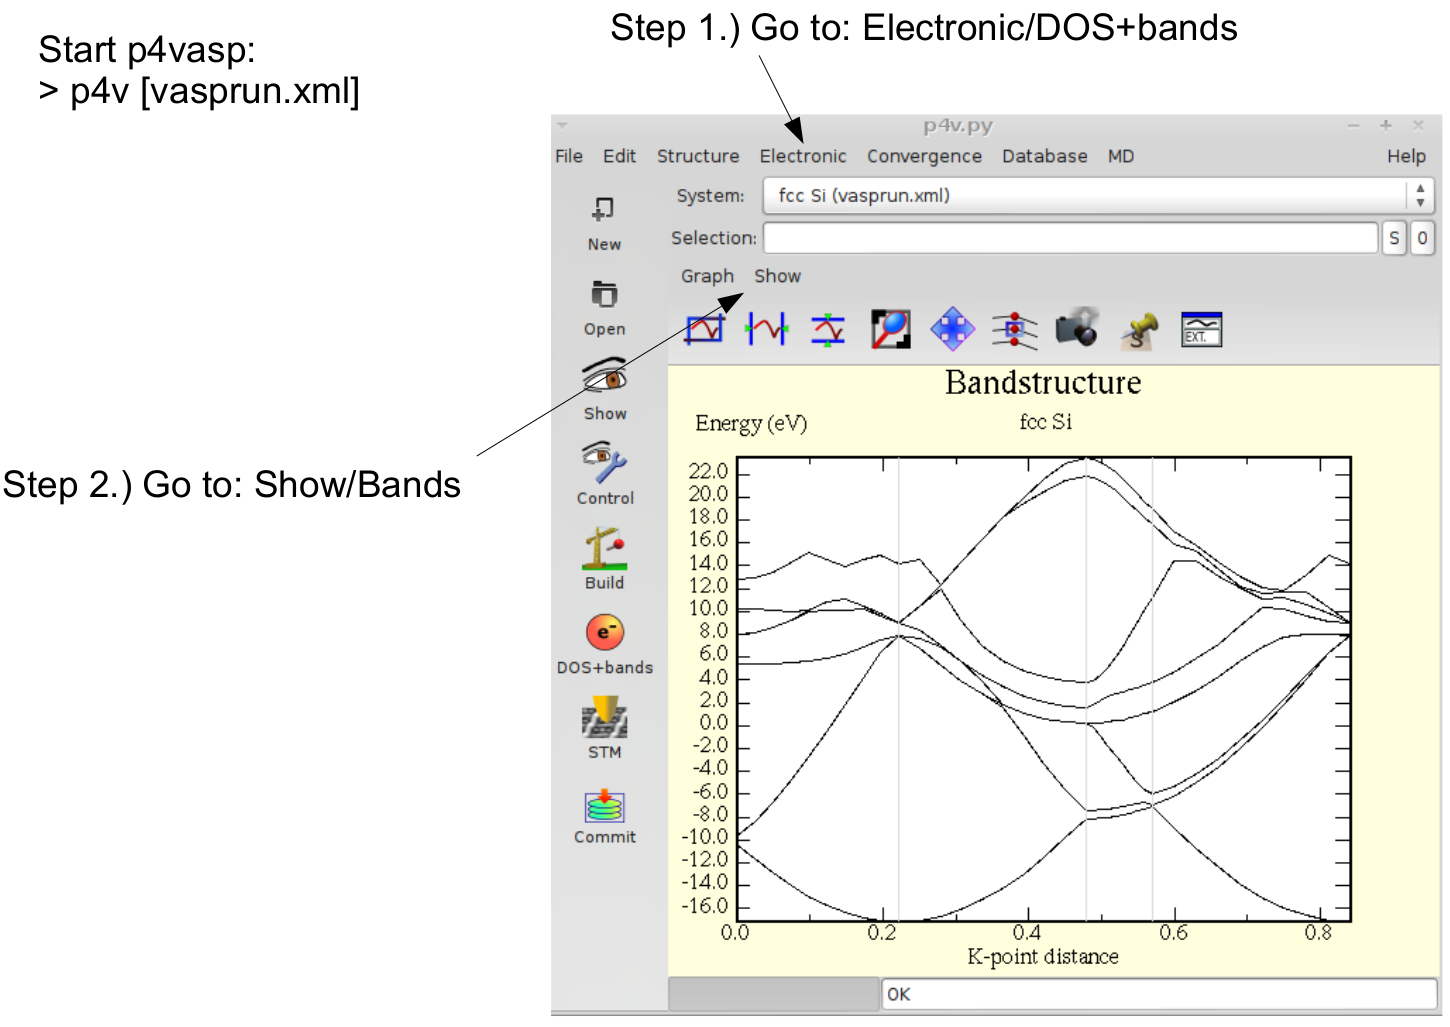
\includegraphics[height=1.7in,width=2.0in,viewport=550 50 1440 915,clip]{Figures/FCC_Si-p4v-Band.png}
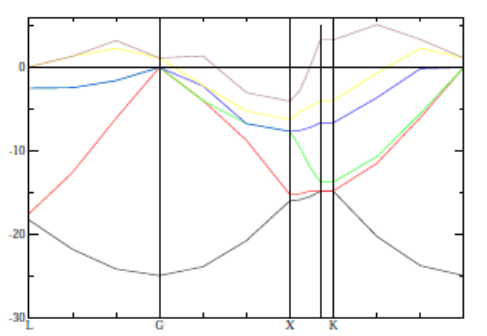
\includegraphics[height=1.5in,width=2.0in,viewport=0 0 500 390,clip]{Figures/FCC_Si-Band.png}
%\caption{\fontsize{7.2pt}{4.2pt}\selectfont{\textrm{The integrated calculator in ASE (Atomic Simulation Environment).}}}%
\label{wiki-FCC-Si}
\end{figure} 
}

\frame
{
	\frametitle{\textrm{结果示例:~\textrm{FCC-Si}}}
\begin{figure}[h!]
\centering
\vspace*{-0.25in}
\includegraphics[height=1.5in,width=2.0in,viewport=0 0 880 600,clip]{Figures/FCC_Si-Band_pymatgen.eps}
\includegraphics[height=1.5in,width=2.0in,viewport=0 0 880 600,clip]{Figures/FCC_Si-DOS_pymatgen.eps}\\
\includegraphics[height=1.5in,width=3.0in,viewport=0 0 830 550,clip]{Figures/FCC_Si-Band_DOS_pymatgen.eps}
%\caption{\fontsize{7.2pt}{4.2pt}\selectfont{\textrm{The integrated calculator in ASE (Atomic Simulation Environment).}}}%
\label{Pymatgen-FCC-Si-Band}
\end{figure} 
}

\frame
{
	\frametitle{基于\textrm{ASE~}和\textrm{Pymatgen~}的自动流程}
	\begin{itemize}
		\item \textcolor{purple}{\textrm{ASE~}}和\textcolor{purple}{\textrm{Pymatgen~}}都是基于\textrm{Python~}开发的,易于整合\\
			\textcolor{magenta}{为实现跨平台的高通量并发式集成计算提供了软件基础}
		\item \textcolor{purple}{\textrm{ASE~}}(建模-计算)
			\begin{enumerate}
				\item 方便的材料建模能力(\textcolor{red}{有扩展余地})
				\item 为多种第一原理和分子动力学软件提供接口,方便各类软件输入参数控制
			\end{enumerate}
		\item \textcolor{purple}{\textrm{Pymatgen~}}(表示-分析)
					\begin{enumerate}
						\item 为计算结果(能带、\textrm{DOS}、相图等)可视化提供了多种工具
						\item 提供数据库管理相关工具(\textcolor{red}{使用方式待了解})
					\end{enumerate}
		\item \textcolor{blue}{当前自动流程的实现,要求用户}
				\begin{enumerate}
					\item 有一定的\textrm{Python~}语言基础
					\item 对\textcolor{purple}{\textrm{ASE~}}和\textcolor{purple}{\textrm{Pymatgen~}}的功能模块有一定了解
				\end{enumerate}
	\end{itemize}
}

\subsection{甲烷催化燃烧机理}
\frame
{
	\frametitle{甲烷氧化的氧交换机制}
\begin{figure}[h!]
\centering
\vskip -12pt
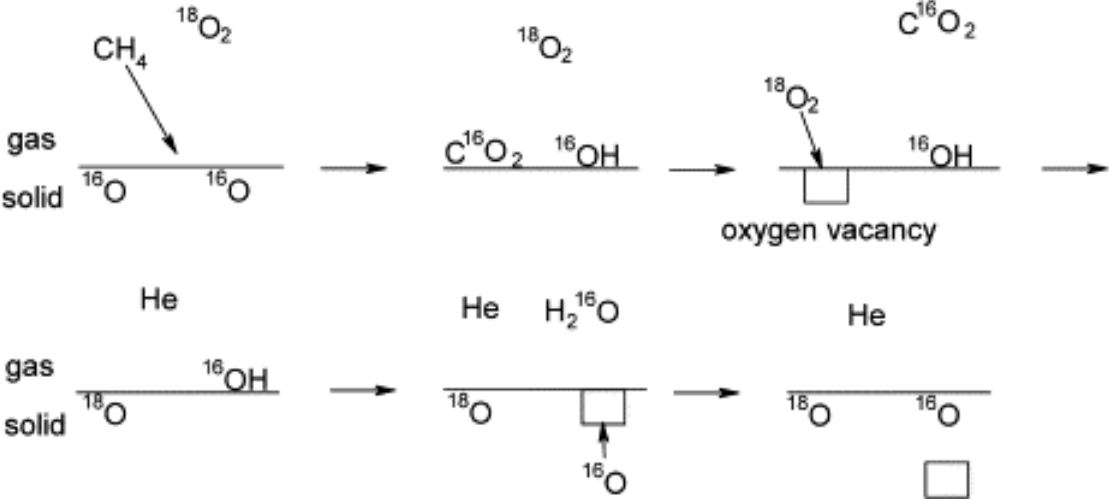
\includegraphics[height=0.8in]{Figures/Oxygen_exchange_mechanism_for_CH4_oxidation.png}
\caption{\fontsize{5.5pt}{4.2pt}\selectfont{催化剂表面甲烷氧化的氧交换过程示意}}%
\label{CH4_comp_mechan}
\end{figure}
\vskip -10pt
	{\fontsize{9.5pt}{11pt}\selectfont
\begin{displaymath}
	\begin{array}{ll}
		\mathrm{Step~1.1}\quad~&\ch{O2(g)}+{\ast}\ch{<=>}\ch{O2}^{\ast} \\
		\mathrm{Step~1.2}\quad~&\ch{O_2}^{\ast}+{\ast}\ch{<=>}2\ch{O}^{\ast} \\
		\mathrm{Step~2.1}\quad~&\ch{CH4(g)}+{\ast}+{\ast}\ch{->}\ch{CH3}^{\ast}+\ch{H}^{\ast} \\
		\mathrm{Step~2.2}\quad~&\ch{CH4(g)}+\ch{O}^{\ast}+{\ast}\ch{->}\ch{CH3}^{\ast}+\ch{OH}^{\ast} \\
		\mathrm{Step~2.3}\quad~&\ch{CH4(g)}+\ch{O}^{\ast}+\ch{O}^{\ast}\ch{->}\ch{CH3O}^{\ast}+\ch{OH}^{\ast} \\
		\mathrm{Step~3}\quad~&\ch{C}^{\ast}+\ch{O}^{\ast}\ch{<=>}\ch{CO}^{\ast}+{\ast} \\
		\mathrm{Step~4}\quad~&\ch{CO}^{\ast}+\ch{O}^{\ast}\ch{<=>}\ch{CO2}^{\ast}+{\ast} \\
		\mathrm{Step~5}\quad~&2\ch{OH}^{\ast}\ch{<=>}\ch{H2O}^{\ast}+\ch{O}^{\ast} \\
		\mathrm{Step~6}\quad~&\ch{H2O}^{\ast}\ch{<=>}\ch{H2O}+{\ast} \\
		\mathrm{Step~7}\quad~&\ch{CO2}^{\ast}\ch{<=>}\ch{CO2}+{\ast} \\
		\mathrm{Step~8}\quad~&\ch{CO}^{\ast}\ch{<=>}\ch{CO}+{\ast}
	\end{array}
\end{displaymath}}
}

\frame
{
	\frametitle{贵金属催化剂失活机制}
\begin{figure}[h!]
\centering
\vskip -12pt
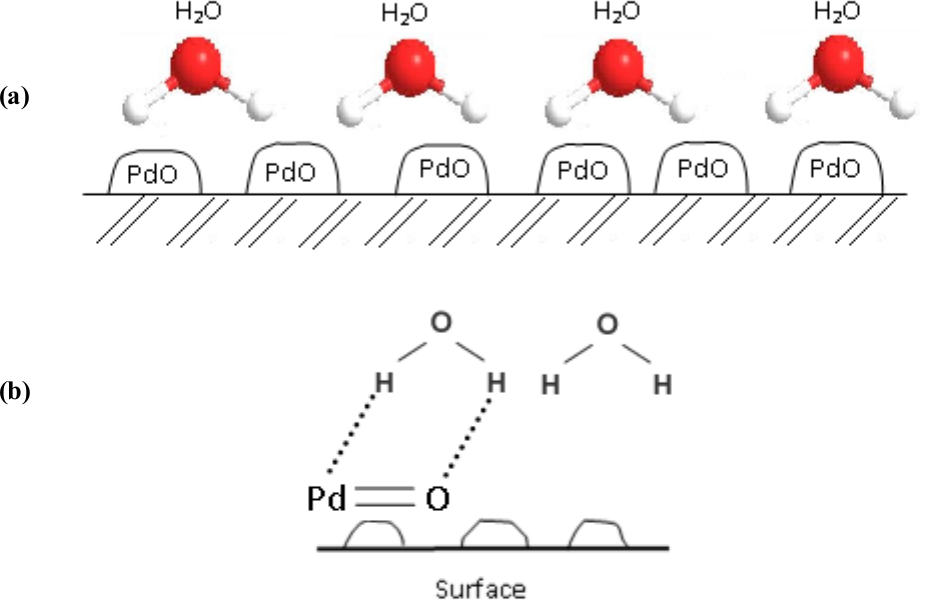
\includegraphics[height=1.2in]{Figures/PdO_H2O.png}\\
\caption{\fontsize{5.5pt}{4.2pt}\selectfont{$\mathrm{H}_2\mathrm{O}$吸附可能引起催化剂失活:~(a)$\mathrm{H}_2\mathrm{O}$吸附;(b)生成$\mathrm{Pd(OH)}_2$导致失活}}%
\label{PdO_H2O}
\end{figure}
\begin{table}[!h]
\tabcolsep 0pt \vspace*{-20pt}
%\begin{center}
\centering
\caption{\textrm{\fontsize{5.5pt}{7.2pt}\selectfont{$\mathrm{CH}_4$第一个\textrm{C-H}键断裂活化能与相应的键长、反应坐标中过渡态对应的虚频}.}}\label{Table-CH}
\vskip -12pt
\def\temptablewidth{0.92\textwidth}
\renewcommand\arraystretch{0.8} %表格宽度控制(普通表格宽度的两倍)
\rule{\temptablewidth}{1pt}
\begin{tabular*} {\temptablewidth}{@{\extracolsep{\fill}}c@{\extracolsep{\fill}}c@{\extracolsep{\fill}}c@{\extracolsep{\fill}}c@{\extracolsep{\fill}}c}
%-------------------------------------------------------------------------------------------------------------------------
	&\multicolumn{2}{c}{\fontsize{7.5pt}{7.2pt}\selectfont{$\mathrm{G}^{\neq}~(\mathrm{eV})$}}	&{\fontsize{7.5pt}{7.2pt}\selectfont{\textrm{d(C-H)}}} &{\fontsize{7.5pt}{7.2pt}\selectfont{\textrm{IMG}}} \\\cline{2-3}
	&\fontsize{7.2pt}{7.2pt}\selectfont{\textrm{PBE}} &{\fontsize{7.2pt}{7.2pt}\selectfont{\textrm{HSE}}} &{\fontsize{7.2pt}{7.2pt}\selectfont{(\textrm{\AA})}} &{\fontsize{7.2pt}{7.2pt}\selectfont{($\mathrm{cm}^{-1}$)}} \\\hline
	\fontsize{7.5pt}{7.2pt}\selectfont{{\textrm{H-ZSM-5}}} &\fontsize{7.5pt}{7.2pt}\selectfont{\textrm{2.86}} &\fontsize{7.5pt}{7.2pt}\selectfont{\textrm{2.40}} &\fontsize{7.5pt}{7.2pt}\selectfont{\textrm{1.431}} &\fontsize{7.5pt}{7.2pt}\selectfont{\textrm{1126.17}}\\
	\fontsize{7.5pt}{7.2pt}\selectfont{{$[\mathrm{AlO}_2]\mathrm{Pd}$-\textrm{H-ZSM-5}}} &\fontsize{7.5pt}{7.2pt}\selectfont{\textrm{1.39}} &\fontsize{7.5pt}{7.2pt}\selectfont{\textrm{2.00}} &\fontsize{7.5pt}{7.2pt}\selectfont{\textrm{1.686}} &\fontsize{7.5pt}{7.2pt}\selectfont{\textrm{899.81}}\\
	\fontsize{7.5pt}{7.2pt}\selectfont{{$[\mathrm{AlO}_2]\mathrm{PdOH}$-\textrm{H-ZSM-5}}} &\fontsize{7.5pt}{7.2pt}\selectfont{\textrm{1.04}} &\fontsize{7.5pt}{7.2pt}\selectfont{\textrm{1.23}} &\fontsize{7.5pt}{7.2pt}\selectfont{\textrm{1.296}} &\fontsize{7.5pt}{7.2pt}\selectfont{\textrm{812.50}}\\
	\fontsize{7.5pt}{7.2pt}\selectfont{{$[\mathrm{AlO}_2]\mathrm{Pd}(\mathrm{OH})_2$-\textrm{H-ZSM-5}}} &\fontsize{7.5pt}{7.2pt}\selectfont{\textrm{1.42}} &\fontsize{7.5pt}{7.2pt}\selectfont{\textrm{1.46}} &\fontsize{7.5pt}{7.2pt}\selectfont{\textrm{1.363}} &\fontsize{7.5pt}{7.2pt}\selectfont{\textrm{793.60}}\\
	\fontsize{7.5pt}{7.2pt}\selectfont{{$[\mathrm{AlO}_2]\mathrm{Pd}[\mathrm{AlO}_2]$-\textrm{H-ZSM-5}}} &\fontsize{7.5pt}{7.2pt}\selectfont{\textrm{2.67}} &\fontsize{7.5pt}{7.2pt}\selectfont{\textrm{2.73}} &\fontsize{7.5pt}{7.2pt}\selectfont{\textrm{1.611}} &\fontsize{7.5pt}{7.2pt}\selectfont{\textrm{683.43}}\\
\end{tabular*}
\rule{\temptablewidth}{1pt}
%\end{center}
\end{table}
}

\frame
{
	\frametitle{非金属盐催化剂活性提升}
\begin{minipage}[b]{0.32\linewidth}
\begin{figure}[h!]
\centering
\vskip 30pt
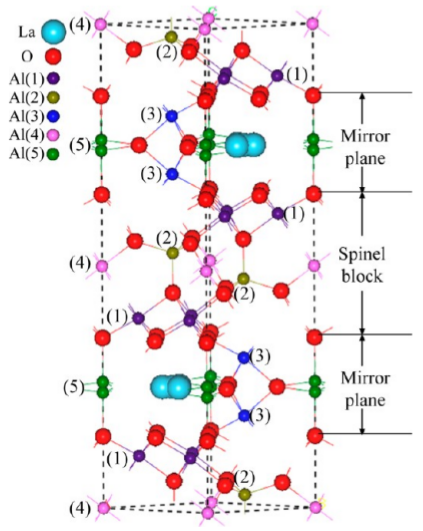
\includegraphics[height=1.62in]{Figures/MAl_12O_19_MP-type_Cat.png}\\
\caption{\fontsize{6.5pt}{4.2pt}\selectfont{\textrm{MP}型\textrm{La}-六铝酸盐.}}%
\label{MP-type}
\end{figure}
\end{minipage}
\begin{minipage}[b]{0.65\linewidth}
\begin{table}[!h]
\tabcolsep 0pt \vspace*{-85pt}
%\begin{minipage}{\0.95\textwidth}
%\begin{center}
\centering
\caption{\textrm{\fontsize{6.5pt}{4.2pt}\selectfont{六铝酸镧原胞中\textrm{Fe}离子取代位点对晶格能的影响.}}}\label{Table-MP-La}
\vskip -5pt
\def\temptablewidth{1.00\textwidth}
\renewcommand\arraystretch{0.8} %表格宽度控制(普通表格宽度的两倍)
\rule{\temptablewidth}{1pt}
\begin{tabular*} {\temptablewidth}{@{\extracolsep{\fill}}c@{\extracolsep{\fill}}c@{\extracolsep{\fill}}c@{\extracolsep{\fill}}c@{\extracolsep{\fill}}c@{\extracolsep{\fill}}c}
%-------------------------------------------------------------------------------------------------------------------------
	\fontsize{4.5pt}{4.2pt}\selectfont{\textrm{Crystal}} &\fontsize{4.5pt}{4.2pt}\selectfont{\textrm{Substituted}}	&\fontsize{4.5pt}{4.2pt}\selectfont{\textrm{Lattice-energy}} & & & \\
	\fontsize{4.5pt}{4.2pt}\selectfont{\textrm{Structure}} &\fontsize{4.5pt}{4.2pt}\selectfont{\textrm{Sites}}	&\fontsize{4.5pt}{4.2pt}\selectfont{\textrm{(eV)}} &\fontsize{4.5pt}{4.2pt}\selectfont{\textit{a}(\textrm{\AA})} &\fontsize{4.5pt}{4.2pt}\selectfont{\textit{b}(\textrm{\AA})} &\fontsize{4.5pt}{4.2pt}\selectfont{\textit{c}(\textrm{\AA})} \\\hline
	\fontsize{4.5pt}{4.2pt}\selectfont{\textrm{spinel block}} &\fontsize{4.5pt}{4.2pt}\selectfont{\textrm{Al(1)}} &\fontsize{4.5pt}{4.2pt}\selectfont{\textrm{-480.56}} &\fontsize{4.5pt}{4.2pt}\selectfont{\textrm{5.60}} &\fontsize{4.5pt}{4.2pt}\selectfont{\textrm{5.60}} &\fontsize{4.5pt}{4.2pt}\selectfont{\textrm{22.04}}\\
	&\fontsize{4.5pt}{4.2pt}\selectfont{\textrm{Al(2)}} &\fontsize{4.5pt}{4.2pt}\selectfont{\textrm{-481.49}} &\fontsize{4.5pt}{4.2pt}\selectfont{\textrm{5.60}} &\fontsize{4.5pt}{4.2pt}\selectfont{\textrm{5.60}} &\fontsize{4.5pt}{4.2pt}\selectfont{\textrm{22.05}}\\
	&\fontsize{4.5pt}{4.2pt}\selectfont{\textrm{Al(4)}} &\fontsize{4.5pt}{4.2pt}\selectfont{\textrm{-480.97}} &\fontsize{4.5pt}{4.2pt}\selectfont{\textrm{5.60}} &\fontsize{4.5pt}{4.2pt}\selectfont{\textrm{5.60}} &\fontsize{4.5pt}{4.2pt}\selectfont{\textrm{21.98}}\\
	\fontsize{4.5pt}{4.2pt}\selectfont{\textrm{mirror plane}} &\fontsize{4.5pt}{4.2pt}\selectfont{\textrm{Al(3)}} &\fontsize{4.5pt}{4.2pt}\selectfont{\textrm{-480.51}} &\fontsize{4.5pt}{4.2pt}\selectfont{\textrm{5.61}} &\fontsize{4.5pt}{4.2pt}\selectfont{\textrm{5.61}} &\fontsize{4.5pt}{4.2pt}\selectfont{\textrm{22.23}}\\
	&\fontsize{4.5pt}{4.2pt}\selectfont{\textrm{Al(5)}} &\fontsize{4.5pt}{4.2pt}\selectfont{\textrm{-480.72}} &\fontsize{4.5pt}{4.2pt}\selectfont{\textrm{5.62}} &\fontsize{4.5pt}{4.2pt}\selectfont{\textrm{5.62}} &\fontsize{4.5pt}{4.2pt}\selectfont{\textrm{22.06}}\\
	\multicolumn{3}{c}{\fontsize{4.5pt}{4.2pt}\selectfont{\textrm{initial value set for unsubstituted La-MP}}} &\fontsize{4.5pt}{4.2pt}\selectfont{\textrm{5.59}} &\fontsize{4.5pt}{4.2pt}\selectfont{\textrm{5.59}} &\fontsize{4.5pt}{4.2pt}\selectfont{\textrm{21.96}}
\end{tabular*}
\rule{\temptablewidth}{1pt}
%\end{minipage}
%\end{center}
\end{table}
\end{minipage}
}

\section{面向催化材料模拟的软件开发}
\frame
{
	\frametitle{适应异质界面催化模拟自动流程软件开发}
\begin{minipage}[b]{0.55\linewidth}
	\begin{itemize}
		\item \fontsize{8.0pt}{4.2pt}\selectfont{适用于异质界面的高通量材料计算自动流程软件架构}
\begin{figure}[h!]
\centering
\hskip -35pt
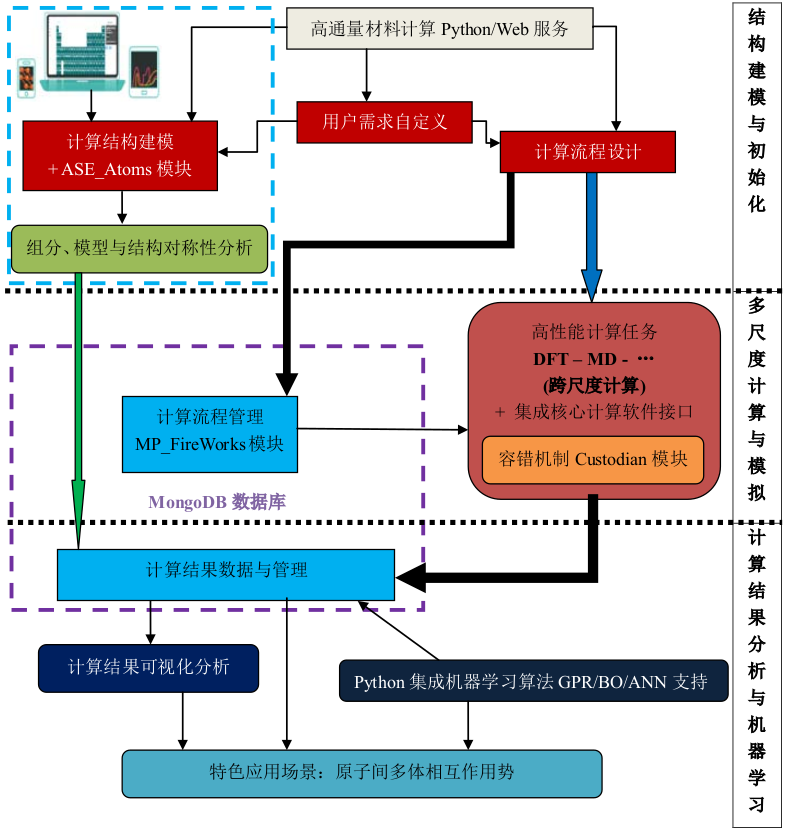
\includegraphics[height=2.18in]{Figures/MP_comp_BCC.png}
%\caption{\fontsize{6.5pt}{4.2pt}\selectfont{适应多体相互作用的高通量计算流程结构示意}}%
\label{MP_comp_BCC}
\end{figure}
	\end{itemize}
\end{minipage}
~
\begin{minipage}[b]{0.33\linewidth}
\begin{itemize}
	\item 设计合理完善的程序流程:~利用\textrm{MongoDB}支持的\textrm{FireWorks}计算流程管理%,由微观尺度\textrm{DFT}计算获得介观或宏观尺度的计算物性或者使不同尺度的计算结果更好地实现耦合自洽
	\item \textcolor{magenta}{机器学习}:~优化电子计算结果,获得\textrm{MD}尺度力场,\textrm{DFT-MD}耦合%,获得\textrm{MD}尺度下准确的多体相互作用的力场函数。
\end{itemize}
\end{minipage}
}

\frame
{
	\frametitle{\rm{DFT-MD}耦合:~催化反应机理模拟流程}
\begin{enumerate}
	\item \fontsize{8.7pt}{6.2pt}\selectfont{\textrm{FireWorks}流程框架支持初始\textrm{DFT}计算并发}
	%\item 为\textrm{DFT}尺度下的原子间相互作用,启动并发式\textrm{Kohn-Sham}方程求解和化学反应动力学(反应通道)计算
	\item \fontsize{8.7pt}{6.2pt}\selectfont{筛选活化能最小的反应通道}%(\textrm{DFT-MD}尺度筛选)
%	\item \textrm{DFT}尺度下,多种结构的反应活化能计算,根据活化能确定可能的决速步
	\item \fontsize{8.7pt}{6.2pt}\selectfont{优化决速步原子间相互作用函数}%(\textrm{DFT-MD}跨尺度耦合)
	\item \fontsize{8.7pt}{6.2pt}\selectfont{求解原子的\textrm{MD}运动方程}
	\item \fontsize{8.7pt}{6.2pt}\selectfont{经\textrm{MD}模拟后确定当前体系各原子结构,返回决速步,\textrm{DFT}再次计算活化能}
	\item \fontsize{8.7pt}{6.2pt}\selectfont{迭代循环,筛选出可能的决速步,得到稳定的催化燃烧反应动力学流程,直至收敛}
\end{enumerate}
\begin{figure}[h!]
\centering
\vskip -2pt
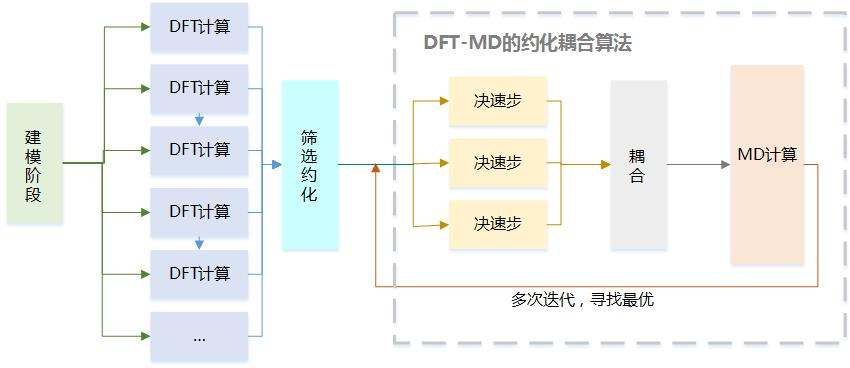
\includegraphics[height=1.05in]{Figures/CH4_complex_machine.png}
\hskip 1pt
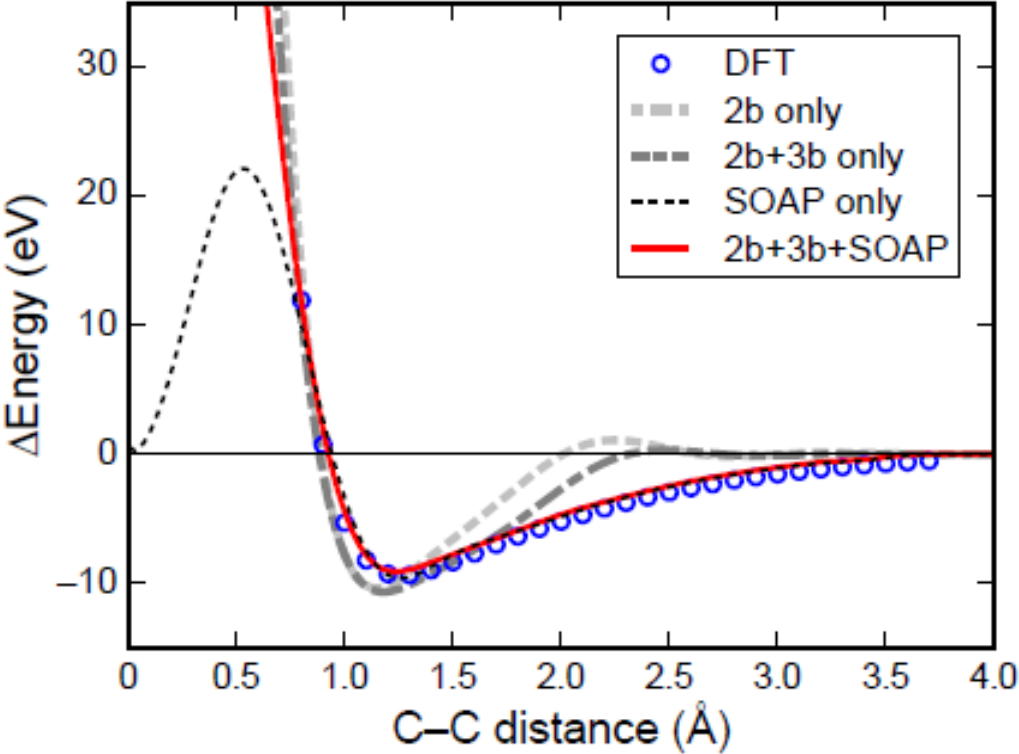
\includegraphics[height=1.05in]{Figures/poten-TiO2.png}%}
\caption{\fontsize{5.5pt}{4.2pt}\selectfont{面向催化燃烧反应动力学机理模拟的计算自动流程示意图}}%
\label{CH4_comp_BCC}
\end{figure}
}

\frame
{
	\frametitle{\rm{DFT-MD}耦合:~复杂体系的原子相互作用势分析}
	\begin{itemize}
		\item \textrm{DFT}计算获得有限尺度原子间相互作用,无法支持\textrm{MD}和反应动力学的规模
		\item \textcolor{magenta}{\textrm{DFT-MD}耦合}\\
			机器学习方法优化\textrm{DFT}的原子相互作用,得到更精确的\textrm{MD}尺度的原子力场
		\item 支持\textrm{MD}尺度下的材料物性模拟
	\end{itemize}
\begin{figure}[h!]
\centering
\vskip -5pt
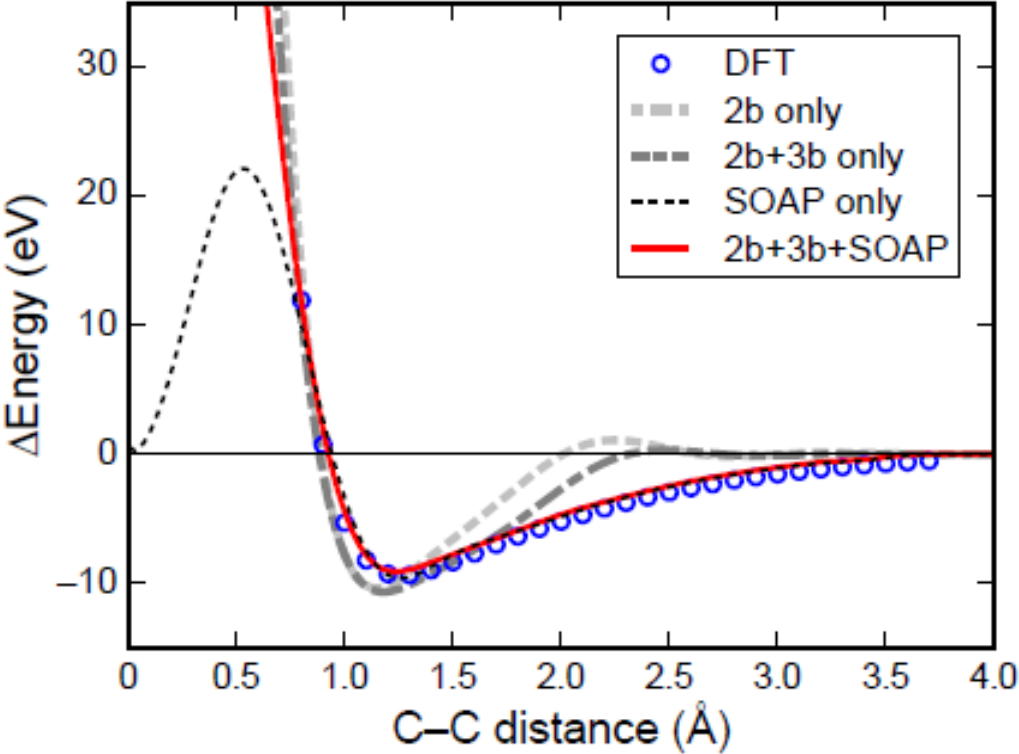
\includegraphics[height=1.2in]{Figures/poten-TiO2.png}%}
\caption{\fontsize{7.5pt}{6.2pt}\selectfont{\textrm{ANN}优化的$\ch{TiO2}$表面的\textrm{C-C}相互作用势能面曲线,对比\textrm{DFT}结果(蓝色).}}%
\label{ANN-poten-TiO2}
\end{figure}
}

%\begin{thebibliography}{99}
%-----------------------------------------------------------------------------------------------------------------------------------------------------------------------%
%\frame
%{
%\frametitle{主要参考资料}
%	\bibitem{Origin-1}网络流传资料:~\textrm{Origin~}图形绘制及曲线拟合.ppt\\{\footnotesize\url{https://wenku.baidu.com/view/7e7c775de2bd960591c67705.html}}					%
%	\bibitem{Origin-2}网络流传资料:~\textrm{Origin~}图形绘制基础入门及曲线拟合.ppt\\{\footnotesize\url{https://wenku.baidu.com/view/d2b85773f46527d3240ce05e.html}}					%
%	\bibitem{Origin-3}网络流传资料:~{\textit{方东明}},~\textrm{Origin~8.0~}二维图形绘制制详解实例和教程.pdf\\{\footnotesize\url{https://wenku.baidu.com/view/eaf64026bd64783e09122b66.html}}					%
%	\bibitem{Origin-4}\textrm{Origin~}官网视频教程:\\{\footnotesize\url{http://www.originlab.com/index.aspx?go=SUPPORT/VideoTutorials}}					%
%	\bibitem{Matlab-1}网络流传资料:~\textrm{Matlab~}绘制曲线的方法.ppt\\{\footnotesize\url{https://wenku.baidu.com/view/dad6257a02768e9951e738e1.html}}					%
%\nocite*{}
%}

%\frame
%{
%\frametitle{发展统一理论框架下的材料计算程序}
%\begin{itemize}
%	\item
%\end{itemize}
%}


%-----------------------------------------------------------Beamer下不建议使用bib,因为涉及分页--------------------------------------------------------------------------%
%{\small
%\phantomsection\addcontentsline{toc}{section}{Bibliography}	 %直接调用\addcontentsline命令可能导致超链指向不准确,一般需要在之前调用一次\phantomsection命令加以修正	%
%\bibliography{Myref}																			%
%\bibliographystyle{mybib}																		%
%  \nocite{*}																				%
%}

%------------------------------------------------------------------------------------------------------------------------------------------------------------------------------%


%-------------------------------------------------------------------------Thanks------------------------------------------------------------------------------------------------
%\section{致谢}
%\frame
%{
%\frametitle{致$\quad$谢}
%\begin{itemize}
%    \setlength{\itemsep}{20pt}
%  \item 感谢本团队高兴誉、吴泉生、宋红州等各位老师参与的讨论
%  \item 感谢莫所长、宋主任以及软件中心各位老师和同事
%  \item 感谢王崇愚先生的帮助
%\end{itemize}
%}

%-------------------------------------------------------------------------------------------------------------------------------------------------------------------------------

\logo{}									%不显示logo
\frame
{
\vskip 60 pt
%\hskip 10pt \textcolor{blue}{\Huge 感谢答辩委员会各位老师\,\textrm{!}}\\
\vskip 35 pt
\hskip 60pt \textcolor{blue}{\Huge 谢谢大家\:!}
%\vskip 15 pt
%\hskip 40pt \textcolor{blue}{\Huge \textrm{for your attention\:!}}
}

%-------------------------------------------------------------------------------------------------------------------------------------------------------------------------------

\clearpage
%\end{CJK*}
\end{document}
%\frame
%{
%\frametitle{发展统一理论框架下的材料计算程序}
%\begin{itemize}
%	\item
%\end{itemize}
%}

%\appendix
%------------------------------------------------------------------------Reference----------------------------------------------------------------------------------------------
%\begin{thebibliography}{99}
%-----------------------------------------------------------------------------------------------------------------------------------------------------------------------%
%\frame
%{
%\frametitle{主要参考文献}
%{\small
%\bibitem{Singh_Book}\textrm{D. J. Singh. \textit{Plane Wave, PseudoPotential and the LAPW method} (Kluwer Academic, Boston,USA, 1994)}					%
%  \nocite{*}																				%
%}
%}
%\end{thebibliography}
\begin{thebibliography}{99}
\frame
{
\frametitle{主要参考文献}
\fontsize{7.5pt}{3.9pt}\selectfont{
%	\bibitem{Huang_Han}黄昆\:原著、韩汝琦\:改编, {\textit{固体物理学}}\:高等教育出版社, 北京, 1988
%	\bibitem{Xie_Lu}谢希德、陆栋\:主编, {\textit{固体能带理论}}\:复旦大学出版社, 上海, 1998
%	\bibitem{url_Mater_Genome}\textrm{\url{https://www.whitehouse.gov/sites/default/files/microsites/ostp/materials_genome_initiative-final.pdf}}
	\bibitem{CMS49-299_2010}\textrm{W. Setyawan and S. Curtarolo \textit{Comp. Mater. Sci.}, \textbf{49} (2010), 299}
	\bibitem{CMS50-2295_2011}\textrm{A. Jain, G. Hautier, C. J. Moore, S. P. Ong, C. C. Fischer, T. M. Kristin, K. A. Persson and G. Ceder \textit{Comp. Mater. Sci.}, \textbf{50} (2011), 2295}
	\bibitem{unpublished}\textrm{D. Gunter, S. Cholia, A. Jain, M. Kocher, K. Persson, L. Ramakrishnan, S. P. Ong and G. Ceder. \textit{Community Accessible Datastore of High-Throughput Calculations: Experiences from the Materials Project} (unpublished)}
	\bibitem{CMS58-227_2012}\textrm{S. Curtarolo, W. Setyawan, S. Wang, J. Xue, K. Yang, R. H. Taylor, L. J. Nelson, G. L. Hart, S. Sanvito, M. Buongiorno-Nardelli, N. Mingo and O. Levy \textit{Comp. Mater. Sci.}, \textbf{58} (2012), 227}
	\bibitem{CMS97-209_2015}\textrm{S. P. Ong, S. Cholia, A. Jain, M. Brafman, D. Gunter, G. Ceder and K. A. Persson. \textit{Comp. Mater. Sci.}, \textbf{97} (2015), 209}
	\bibitem{url_QMIP}\textrm{\url{http://www.qmip.org/qmip.org/Welcome.html}}
	\bibitem{JPCL2-2241_2011}\textrm{J. Hachmann, R. Olivares-Amaya, S. Atahan-Evrenk, C. Amador-Bedolla, R. S. S$\acute{a}$nchez-Carrera, A. Gold-Parker, L. Vogt, A. M. Brockway and A. Aspuru-Guzik \textit{J. Phys. Chem. Lett.}, \textbf{2} (2011), 2241}
}
\nocite*{}
}
\end{thebibliography}
%{\small
%\phantomsection\addcontentsline{toc}{section}{Bibliography}	 %直接调用\addcontentsline命令可能导致超链指向不准确,一般需要在之前调用一次\phantomsection命令加以修正	%
%\bibliography{Myref}																			%
%\bibliographystyle{mybib}																		%
%  \nocite{*}																				%
%}
%-----------------------------------------------------------------------------------------------------------------------------------------------------------------------%


%-----------------------------------------------------------Beamer下不建议使用bib,因为涉及分页--------------------------------------------------------------------------%
%{\small
%\phantomsection\addcontentsline{toc}{section}{Bibliography}	 %直接调用\addcontentsline命令可能导致超链指向不准确,一般需要在之前调用一次\phantomsection命令加以修正	%
%\bibliography{Myref}																			%
%\bibliographystyle{mybib}																		%
%  \nocite{*}																				%
%}

%------------------------------------------------------------------------------------------------------------------------------------------------------------------------------%

%-------------------------------------------------------------------------Thanks------------------------------------------------------------------------------------------------
%\section{致谢}
%\frame
%{
%\frametitle{致$\quad$谢}
%\begin{itemize}
%    \setlength{\itemsep}{20pt}
%  \item 感谢本团队高兴誉、吴泉生、宋红州等各位老师参与的讨论
%  \item 感谢莫所长、宋主任以及软件中心各位老师和同事
%  \item 感谢王崇愚先生的帮助
%\end{itemize}
%}
%\frame
%{
%	\frametitle{\textrm{PAW Augmentation}}
%\begin{figure}[h!]
%\centering
%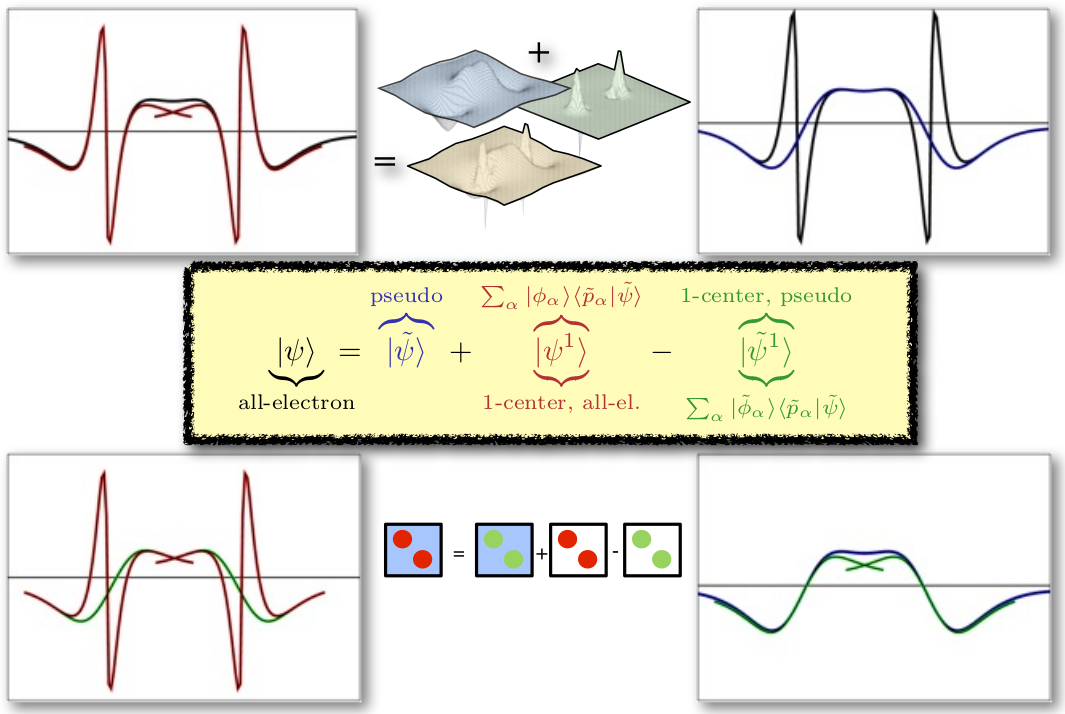
\includegraphics[height=2.3in,width=4.0in,viewport=0 0 1100 745,clip]{Figures/PAW-projector.png}
%\caption{\tiny \textrm{The projector of PAW.}}%(与文献\cite{EPJB33-47_2003}图1对比)
%\label{PAW_projector}
%\end{figure}
%}
%\frame
%{
%	\frametitle{赝势-\textrm{PAW}方法}
%\begin{figure}[h!]
%\centering
%%\hspace*{-0.80in}
%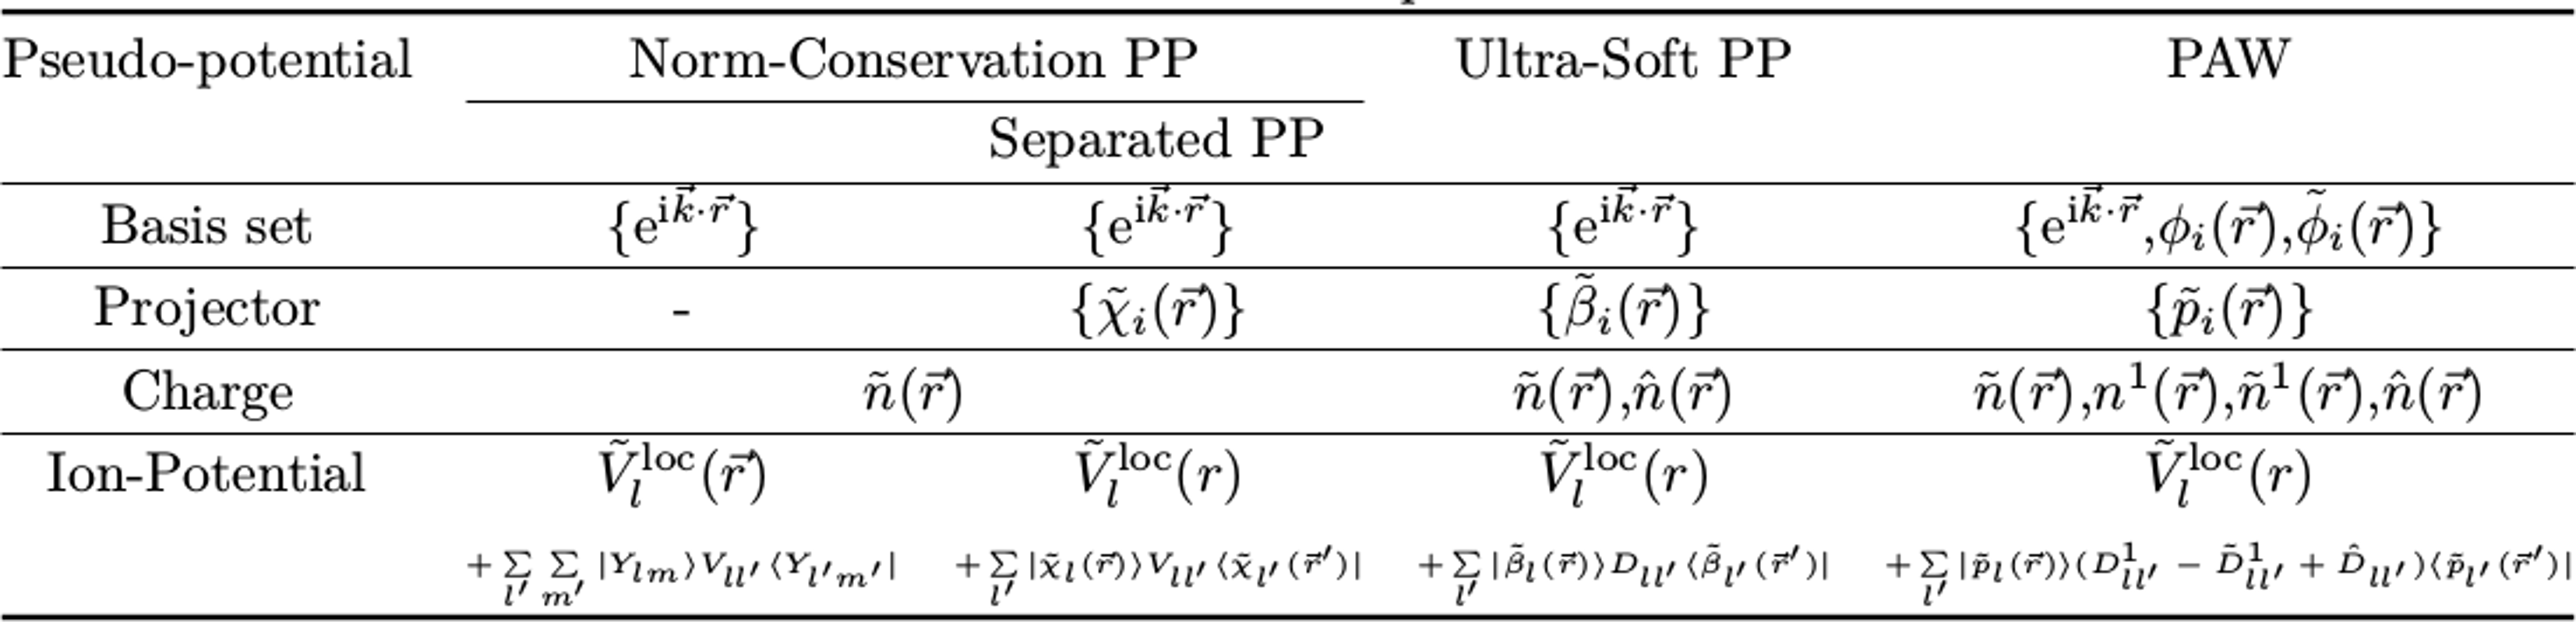
\includegraphics[height=1.0in,width=4.1in,clip]{Figures/Pseudo-Potential.png}
%\caption{\tiny \textrm{The relation of Pseudo potential and PAW.}}%(与文献\cite{EPJB33-47_2003}图1对比)
%\label{Pseudo_Poential}
%\end{figure}
%}
%
\section{\rm{POTCAR}的重构}
\frame
{
	\frametitle{\textrm{VASP}计算的原子数据基础}
	\textrm{POTCAR}提供了\textrm{VASP}计算所需的原子数据,也是实现\textrm{PAW}方法的主要基础
	\begin{itemize}
		\item \textrm{POTCAR}是\textrm{VASP}实现材料精确计算的重要保证\\
			同样都应用\textrm{PAW}方法,\textcolor{blue}{公认\textrm{VASP}较\textrm{QE}、\textrm{ABINIT}等软件的计算精度要高}
		\item \textrm{POTCAR}数据生成依赖较多的可调参数\\
			包括能量参数$\varepsilon_l$、多种截断半径$r_c$、$r_{\mathrm{vloc}}$、$r_{\mathrm{shape}}$、$r_{\mathrm{core}}$
		\item \textcolor{red}{\textrm{POTCAR}数据生成代码是\textrm{VASP}中唯一没有公开的}
		\item 用\textrm{VASP}模拟极端条件下材料物性的能力,受到\textrm{POTCAR}数据的制约
	\end{itemize}
	%文献\cite{PRB59-1758_1999}介绍了\textrm{POTCAR}的主要实现思想

当前研究主要尝试基于开源的\textrm{PAW}赝势生成软件(\textrm{atomPAW}),开发能生成\textrm{POTCAR}原子数据的功能
}

\frame
{
	\frametitle{\textrm{PAW}原子数据集:~\textrm{wave~function}}
	平滑赝原子分波函数
	\begin{displaymath}
		\tilde\phi_{i=Lk}(\vec r)=Y_L(\widehat{\vec r-\vec R})\tilde\phi_{lk}(|\vec r-\vec R|)
	\end{displaymath}
	根据\textrm{RRKJ}赝势构造的思想,赝分波函数由球\textrm{Bessel}函数线性组合\upcite{JPCM6-8245_1994}
	\begin{displaymath}
		\tilde\phi_{lk}(r)=\left\{
		\begin{aligned}
			&\sum_{i=1}^2\alpha_ij_l(q_ir)\quad &r<r_c^l\\
			&\phi_{lk}(r)\quad&r>r_c^l
		\end{aligned}
		\right.
	\end{displaymath}
	调节系数$\alpha_i$和$q_i$赝分波函数$\phi_{lk}(r)$在截断半径$r_c^l$处两阶连续可微
%	投影子波函数$\tilde p_i$由\textrm{Gram-Schmidt}正交条件$\langle\tilde p_i|\tilde\phi_j\rangle=\delta_{ij}$确定
}

\frame
{
	\frametitle{\textrm{PAW}原子数据集:~\textrm{wave~function}}
\begin{figure}[h!]
\centering
\vskip -0.5in
\includegraphics[width=1.5in,height=2.7in,viewport=0 0 350 550, angle=-90, clip]{Figures/WAE_data.eps}
\vskip -0.2in
\includegraphics[height=2.7in,width=1.5in,viewport=0 0 350 550, angle=-90, clip]{Figures/WPS_data.eps}
\caption{\tiny \textrm{The partial wave function.}}%(与文献\cite{EPJB33-47_2003}图1对比)
\label{Wave_Function}
\end{figure}
}

\frame
{
	\frametitle{\textrm{PAW}原子数据集:~\textrm{core~density}}
	\textcolor{blue}{构造赝芯电荷密度$\tilde n_c$}:~在截断半径$r_{\mathrm{core}}$内的定义为
	$$\sum_{i=1,2}B_i\dfrac{\sin(q_ir)}r\quad r<r_{\mathrm{core}}$$
	调节系数$q_i$和$B_i$使得赝芯电荷密度$\tilde n_c(r)$在截断半径$r_{\mathrm{core}}$处的两阶导数连续
\begin{figure}[h!]
\vskip -0.5in
\centering
\hspace*{-0.1in}
\includegraphics[width=1.5in,height=2.35in,viewport=0 0 350 550, angle=-90, clip]{Figures/CORE_data.eps}
\hspace*{-0.7in}
\includegraphics[height=2.35in,width=1.5in,viewport=0 0 350 550, angle=-90, clip]{Figures/PCORE_data.eps}
\caption{\tiny \textrm{The core density.}}%(与文献\cite{EPJB33-47_2003}图1对比)
\label{core_density_Function}
\end{figure}
}

\frame
{
	\frametitle{\textrm{PAW}原子数据集:~$\mathrm{v}_{e\!f\!f}(r)$与$\tilde{\mathrm{v}}_{e\!f\!f}(r)$}
	\textcolor{blue}{原子局域有效势$\mathrm{v}_{e\!f\!f}^a$}
\begin{figure}[h!]
\vskip -0.1in
\centering
\includegraphics[width=1.3in,height=2.4in,viewport=0 0 700 1200, angle=-90, clip]{Figures/POTAE.eps}
\caption{\tiny \textrm{The local atomic effective-Potential.}}%(与文献\cite{EPJB33-47_2003}图1对比)
\label{local_atomic_PP}
\end{figure}
	\textcolor{blue}{构造原子局域赝势$\tilde v_{e\!f\!f}^a$}%(\textcolor{red}{为防止\textrm{ghost band}})
	:%\\
	(在截断半径$r_{\mathrm{loc}}$内的定义)
	$$\tilde v_{e\!f\!f}^a=A\dfrac{\sin(q_{loc}r)}r\quad r<r_{\mathrm{loc}}$$
	其中$q_{loc}$和$A$要求局域赝势在截断半径$r_{\mathrm{loc}}$处连续到一阶导数
}

\frame
{
	\frametitle{\textrm{PAW}原子数据集:~$\mathrm{v}_H[\tilde n_{Zc}]$}
	局域离子赝势$v_H[\tilde n_{Zc}]$可由原子局域赝势去屏蔽得到
	$$v_H[\tilde n_{Zc}]=\tilde v_{e\!f\!f}^a-v_H[\tilde n_a^1+\hat n_a]-v_{\mathrm{XC}}[\tilde n_a^1+\hat n_a+\tilde n_c]$$
\begin{figure}[h!]
\vskip -0.5in
\centering
\hspace*{-0.1in}
\includegraphics[width=1.5in,height=2.35in,viewport=0 0 350 550, angle=-90, clip]{Figures/POTPS_data.eps}
\hspace*{-0.7in}
\includegraphics[height=2.35in,width=1.5in,viewport=0 0 350 550, angle=-90, clip]{Figures/POTPSC_data.eps}
\caption{\tiny \textrm{The pseudo-potential and local ionic pseudo-potential.}}%(与文献\cite{EPJB33-47_2003}图1对比)
\label{pseudo_potential}
\end{figure}
}

\frame
{
	\frametitle{\textrm{PAW}原子数据集:~倒空间$\tilde{\mathrm{v}}_{\mathrm{ion}}^a(G)$}和$\tilde n(G)$
	由势函数由实空间向倒空间的变换关系
	\begin{displaymath}
		\begin{aligned}
%			\textrm{v}(G)=&e^2\int\dfrac{\mathrm{d}^2r}{\mathrm r}\mathrm{e}^{\mathrm{i}\vec G\cdot\vec r}=2\pi e^2\int_0^{\infty}r\mathrm{d}r\int_{-1}^1\mathrm{d}(\cos\theta)\mathrm{e}^{\mathrm{i}Gr\cos\theta}\\
%			=&\dfrac{2\pi e^2}{\mathrm{i}G}\int_0^{\infty}\mathrm{d}r(\mathrm{e}^{\mathrm{i}Gr}-\mathrm{e}^{-\mathrm{i}Gr})=\dfrac{4\pi e^2}G\int_0^{\infty}\mathrm{d}r\sin(Gr)
			\textrm{v}(G)=&\int\mathrm{d}^3r v(r)\mathrm{e}^{\mathrm{i}\vec G\cdot\vec r}=2\pi \int_0^{\infty} v(r)\cdot r~r\mathrm{d}r\int_{-1}^1\mathrm{d}(\cos\theta)\mathrm{e}^{\mathrm{i}Gr\cos\theta}\\
			=&\dfrac{2\pi}{\mathrm{i}G}\int_0^{\infty}v(r)\cdot r~\mathrm{d}r(\mathrm{e}^{\mathrm{i}Gr}-\mathrm{e}^{-\mathrm{i}Gr})=\dfrac{4\pi}G\int_0^{\infty}\sin(Gr)v(r)\cdot r~\mathrm{d}r
		\end{aligned}
	\end{displaymath}
	可将$\mathrm{v}_H[\tilde n_{Zc}]$和$\tilde n(G)$变换为倒空间表示
\begin{figure}[h!]
\vskip -0.12in
\centering
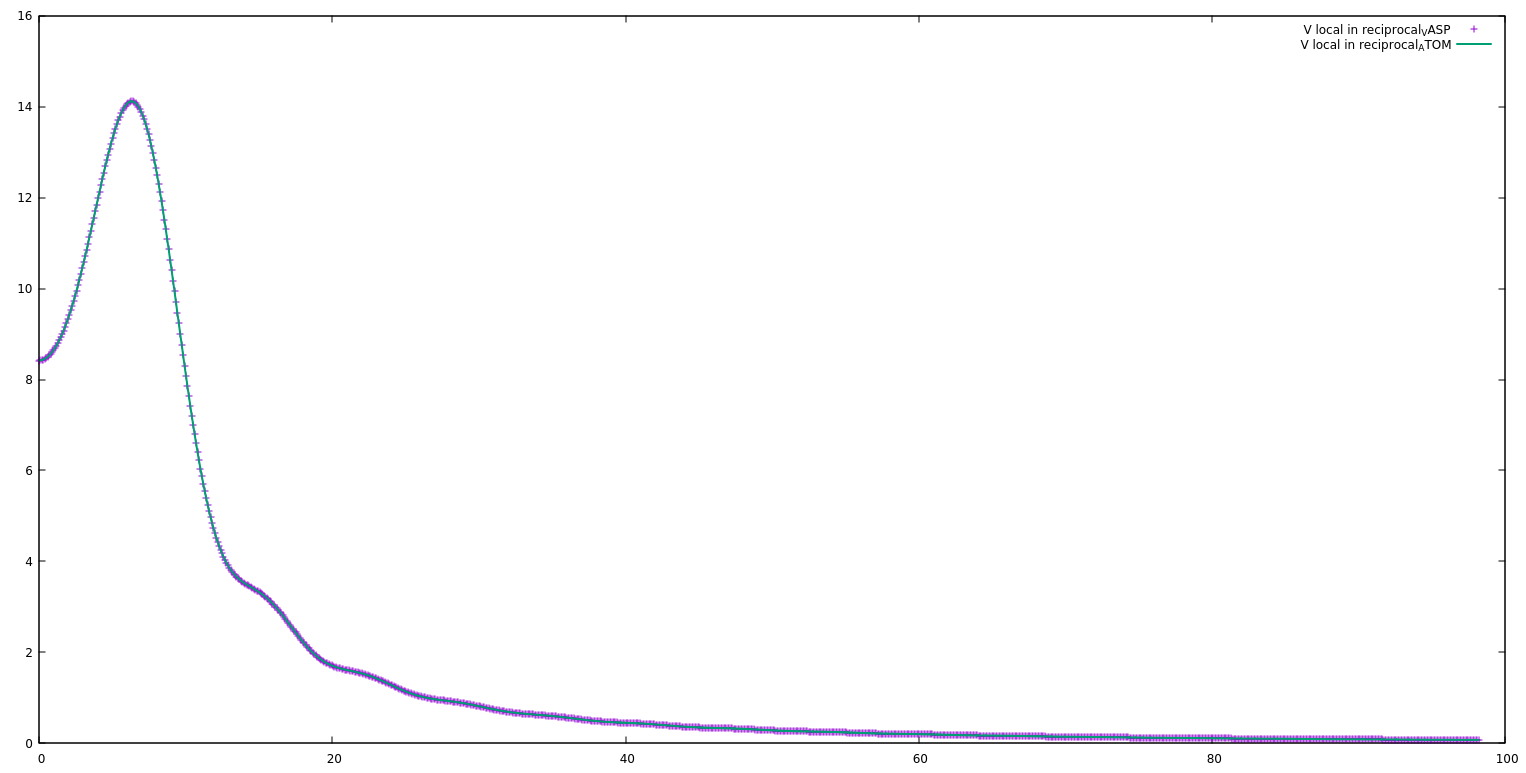
\includegraphics[width=2.5in,height=1.4in,viewport=0 0 1200 630, clip]{Figures/PAW_Vloc_G.png}
\caption{\tiny \textrm{The pseudo-potential in reciprocal space.}}%(与文献\cite{EPJB33-47_2003}图1对比)
\label{pseudo_potential_G}
\end{figure}
}

\section{后续工作}
\frame
{
	\frametitle{后续工作}
	\begin{itemize}
		\item 完成\textrm{POTCAR}的全部原子数据的生成
			\begin{itemize}
   				\setlength{\itemsep}{10pt}
				\item 赝电荷密度$\tilde n_v(r)$在倒空间的表示$\tilde n_v(G)$
				\item 赝芯电荷密度$\tilde n_c(r)$在倒空间的表示$\tilde n_c(G)$
				\item 投影函数在倒空间$\tilde p_l(G)$和实空间(优化)~$\tilde p_l(r)$的表示
				\item \textrm{PAW}方法中引入原子赝势后的修正$\Delta D_{\mathrm{ion}}(r)$
					\begin{displaymath}
						\hspace*{-50pt}\Delta D_{ij}^{\mathrm{ion}}(r)=\langle\phi_i\left|T+V_{e\!f\!f}^a\right|\phi_j\rangle-\langle\tilde\phi_i\left|T+\tilde V_{e\!f\!f}^a\right|\tilde\phi_j\rangle-\int\hat{Q}_{ij}^{00}(r)\tilde{V}_{e\!f\!f}^a(r)\mathrm{d}r 
					\end{displaymath}
			\end{itemize}
		\item 优化原子生成参数,探索适合极端条件(高压)下\textrm{VASP}计算的原子数据集(\textrm{PAW~DataSet})
	\end{itemize}
}

%------------------------------------------------------------------------Reference----------------------------------------------------------------------------------------------
\frame[allowframebreaks]
{
\frametitle{主要参考文献}
{\tiny\textrm{
%\phantomsection\addcontentsline{toc}{section}{Bibliography}	 %直接调用\addcontentsline命令可能导致超链指向不准确,一般需要在之前调用一次\phantomsection命令加以修正	%
%\phantomsection\addcontentsline{toc}{section}{主要参考文献}	 %直接调用\addcontentsline命令可能导致超链指向不准确,一般需要在之前调用一次\phantomsection命令加以修正	%
%\bibliography{Ref_2020-03-04}%
\bibliography{Ref_2020-03-04}%
\bibliographystyle{../ref/mybib}%
}}
%\nocite{*}%
}

%------------------------------------------------------------------------------------------------------------------------------------------------------------------------------%
%\frame
%{
%\frametitle{主要参考文献}
%\begin{thebibliography}{99}
%{\small
%\bibitem{Singh_Book}\textrm{D. J. Singh. \textit{Plane Wave, PseudoPotential and the LAPW method} (Kluwer Academic, Boston,USA, 1994)}					%
%\end{thebibliography}
%  \nocite{*}																				%
%}
%}

%-------------------------------------------------------------------------Thanks------------------------------------------------------------------------------------------------
%\section{致谢}
%\frame
%{
%\frametitle{致$\quad$谢}
%\begin{itemize}
%    \setlength{\itemsep}{20pt}
%  \item 感谢本团队高兴誉、吴泉生、宋红州等各位老师参与的讨论
%  \item 感谢莫所长、宋主任以及软件中心各位老师和同事
%  \item 感谢王崇愚先生的帮助
%\end{itemize}
%}

\logo{}									%不显示logo
\frame
{
\vskip 60 pt
%\hskip 10pt \textcolor{blue}{\Huge 感谢答辩委员会各位老师\,\textrm{!}}\\
\vskip 35 pt
\hskip 60pt \textcolor{blue}{\Huge 谢谢大家\:!}
%\vskip 15 pt
%\hskip 40pt \textcolor{blue}{\Huge \textrm{for your attention\:!}}
}

\appendix
\frame
{
	\frametitle{补偿电荷的构造}
	根据约束条件
	\begin{displaymath}
		\int_{\Omega_c}(n^1-\tilde n^1-\hat n)|\vec r-\vec R|^lY_{lm}^{\ast}(\widehat{\vec r-\vec R})\mathrm{d}\vec r=0
	\end{displaymath}
	定义电荷密度差
	\begin{displaymath}
		Q_{ij}(\vec r)=\phi_i^{\ast}(\vec r)\phi_j(\vec r)-\tilde\phi_i^{\ast}(\vec r)\tilde\phi_j(\vec r)
	\end{displaymath}
	电荷密度差的多极矩为
	\begin{displaymath}
		q_{ij}^L(\vec r)=\int_{\Omega_r}Q_{ij}(\vec r)|\vec r-\vec R|^lY_{lm}^{\ast}(\widehat{\vec r-\vec R})\mathrm{d}\vec r
	\end{displaymath}
	因此,补充电荷的计算为:
	\begin{displaymath}
		\begin{aligned}
			\hat n=\sum_{(i,j),L}\sum_n f_n\langle\tilde\Psi_n|\tilde p_i\rangle\langle\tilde p_j|\Psi_n\rangle\hat Q_{ij}^L(\vec r)\\
			\hat Q_{ij}^L(\vec r)=q_{ij}^Lg_l(|\vec r-\vec R|)Y_{lm}(\widehat{\vec r-\vec R})
		\end{aligned}
	\end{displaymath}
}

\frame
{
	\frametitle{补偿电荷的构造}
	在每个原子球内用球\textrm{Bessel}函数构造补偿电荷$g_l(r)$
	$$g_l(r)=\sum_{i=1}^2\alpha_i^lj_l(q_i^lr)$$
	调节系数$q_i^l$和$\alpha_i^l$使得补偿电荷$g_l(r)$在截断半径$r_{\mathrm{\mathrm{comp}}}$处的数值和前两阶导数值都是0,因此可以选择$q_i^l$使得多极矩
	$$\int_0^{r_{\mathrm{comp}}}g_l(r)r^{l+2}\mathrm{d}r=1$$
	并且有
	$$\dfrac{\mathrm{d}}{\mathrm{d}r}j_l(q_i^lr)\bigg|_{r_{\mathrm{comp}}}=0$$
	设置$\alpha_i^l$,因此$g_l(r_{\mathrm{comp}})=0$

	$\ast$各截断半径确定的参考条件\\
	{\fontsize{6.2pt}{4.2pt}\selectfont{\textcolor{blue}{$r_{\mathrm{rad}}=\max({r_c^l})$,~$r_{pc}\approx r_{\mathrm{rad}}/1.2$,~$r_{loc}<r_{\mathrm{rad}}/1.2$,~$r_{\mathrm{comp}}=r_{\mathrm{rad}}/1.3\sim r_{\mathrm{rad}}/1.2$}}}
}

\frame
{
	\frametitle{双网格技术}
\begin{figure}[h!]
	\vspace{-0.2in}
\centering
%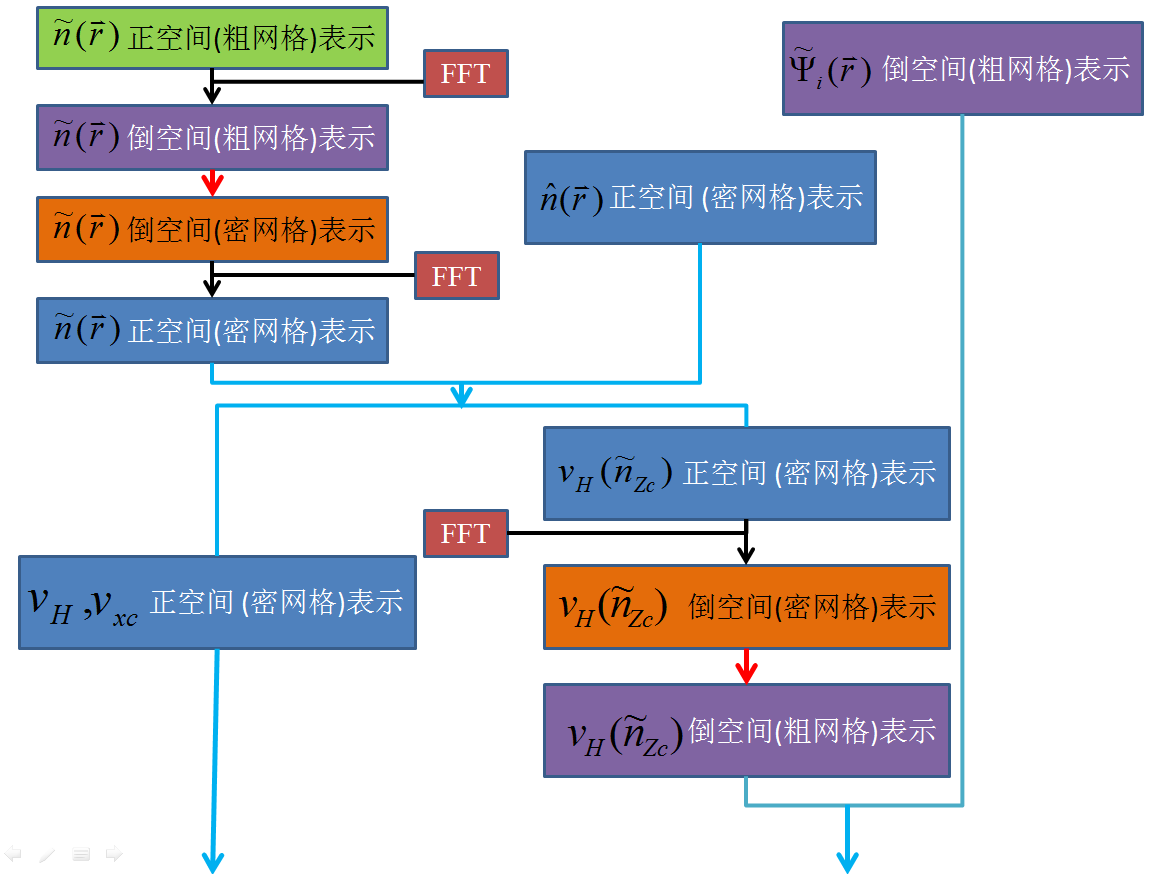
\includegraphics[height=2.7in,width=4.0in,viewport=0 0 1180 875,clip]{Figures/dual_grid.png}
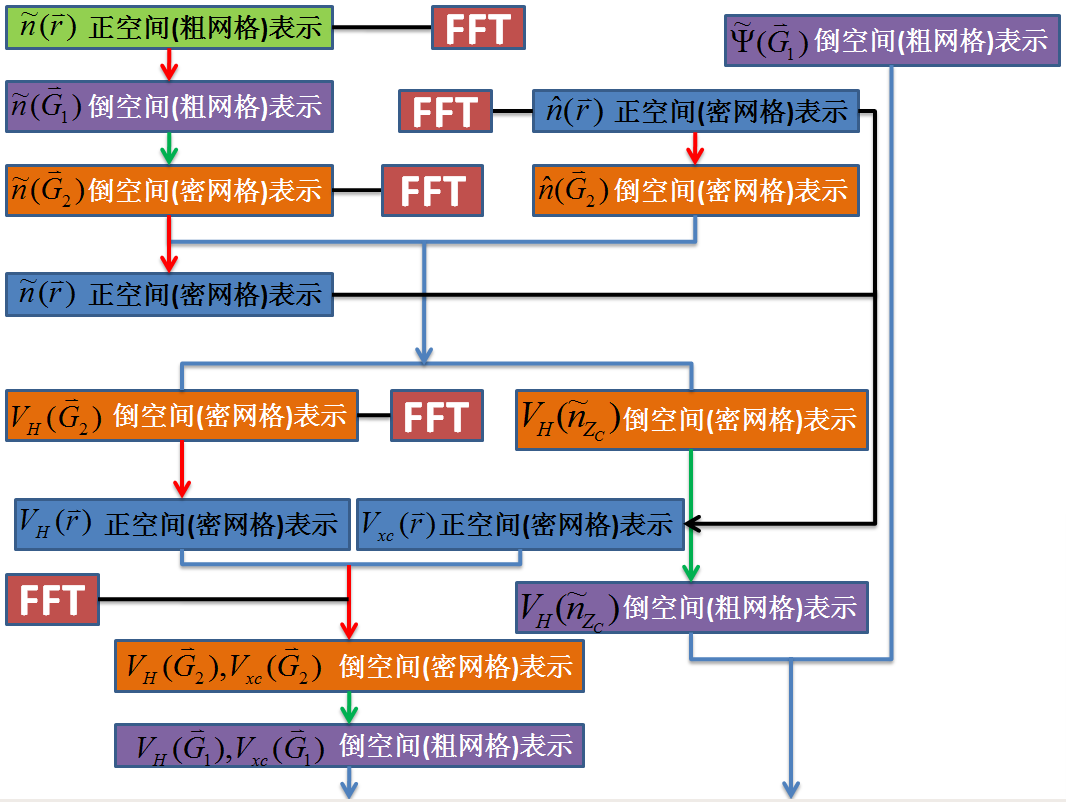
\includegraphics[height=2.7in,width=4.0in,viewport=0 0 800 600,clip]{Figures/dual_grid-2.png}
\caption{\tiny \textrm{The Schematic description of the dual grid technique.}}%(与文献\cite{EPJB33-47_2003}图1对比)
\label{PAW_dualgrid}
\end{figure} 
}

\frame
{
	\frametitle{一维\textrm{FFT}的\textrm{MPI}并行}
\begin{figure}[h!]
	\vspace{-0.15in}
\centering
%\includegraphics[height=2.7in,width=4.0in,viewport=0 0 1180 875,clip]{Figures/dual_grid.png}
\includegraphics[height=1.55in,width=2.2in,viewport=0 10 810 580,clip]{Figures/FFT_para.png}
\vskip 0.5pt
\includegraphics[height=1.2in,width=3.5in,viewport=0 0 1180 550,clip]{Figures/FFT_para-2.png}
\caption{\tiny \textrm{The Schematic description for FFT in MPI.}}%(与文献\cite{EPJB33-47_2003}图1对比)
\label{MPI-FFT}
\end{figure} 
}

\frame
{
	\frametitle{\textrm{VASP}计算的并行实现}
	\begin{itemize}
	     \item 中间层设计:~\textrm{FFT}网格、实空间基组与计算节点的匹配\\
		     \textcolor{magenta}{通过子程序\textrm{mgrid.F}生成中间层,实现并行负载与计算节点分配的匹配,减少\textrm{FFT}变换和实空间并行的节点间通信}
\begin{figure}[h!]
		\vspace{-0.25in}
	\centering
%\includegraphics[height=2.7in,width=4.0in,viewport=0 0 1180 875,clip]{Figures/dual_grid.png}
\includegraphics[height=1.0in,width=4.0in,viewport=0 0 1500 450,clip]{Figures/VASP_FFT-MPI_Reciprocal.png}
\vskip 0.5pt
\includegraphics[height=0.7in,width=4.0in,viewport=0 0 730 150,clip]{Figures/VASP_FFT-MPI_Real.png}
\caption{\tiny \textrm{VASP:~ Reciprocal-Real space layout for grids in MPI.}}%(与文献\cite{EPJB33-47_2003}图1对比)
\label{MPI-FFT}
\end{figure} 
	\end{itemize}
}

%\frame
%{
%\begin{figure}[h!]
%\centering
%\animategraphics[autoplay, loop, height=2.1in]{1}{Figures/Prof_Liu-}{06}{11}
%\label{Prof_Liu}
%\end{figure}
%}
%
%-------------------------------------------------------------------------------------------------------------------------------------------------------------------------------

\clearpage
%\end{CJK*}
\end{document}
